\documentclass{jimis-en}
\pdfoutput=1 %forces arXiv/HAL to compile with PDFLaTeX

% Packages
\usepackage{array}
\usepackage{pgfplots}
\usepackage{graphicx}

% header
\title{Multi-dimensional Urban Network Percolation}


\author[1,2,3,*]{Juste RAIMBAULT}
\affil[1]{UPS CNRS 3611 ISC-PIF, France}
\affil[2]{CASA, UCL, UK}
\affil[3]{UMR CNRS 8504 G{\'e}ographie-cit{\'e}s}
 
% corresponding author with his/her email
\corrauthor{juste.raimbault@polytechnique.edu}

%% Information provided by JIMIS:
%ISSN
% DOI 
\doi{10.18713/JIMIS-ddmmyy-v-a}{}
% reviewing process: first date = submission, second date = acceptance 
\review{Month-in-letters Day Year}{Month-in-letters Day Year}
% Volume and Year of the issue
\publication{N}{YYYY}

%% Information provided by the Editors:
% Issue Title 
\issue{Title of the interdisciplinary issue}
% List of k Editors
\editors{}

\begin{document}

\maketitle

\abstract{Network percolation has recently been proposed as a method to characterize the hierarchical structure of an urban system form the bottom-up. This paper proposes to extend urban network percolation in a multi-dimensional way, to take into account both urban form (spatial distribution of population) and urban functions (here as properties of transportation networks). The method is applied to the European urban system to reconstruct endogenous urban regions. The variable parametrization allows to consider patterns of optimization for two stylized contradictory sustainability indicators (economic performance and greenhouse gases emissions). This suggests a customizable spatial design of policies to develop sustainable territories.}

\keywords{Road network; Multi-dimensional percolation; European urban system; Mega-city region}



\section{Introduction}

\strut
\vspace{-4ex}




\subsection{Towards multidimensional urban network percolation}

The structure of road networks can be used as a proxy to understand its past growth dynamics, but also has a significant impact on the future sustainability of territories it irrigates. Diverse methods to characterize the structure of spatial networks, and more particularly road networks, have been developed in that context. They include classical network indicators such as centralities \citep{crucitti2006centrality} but also more elaborated constructions capturing more realistic processes in terms of street network use \citep{lagesse2015spatial}. Such studies of urban networks are by essence interdisciplinary, or at least imply complementary viewpoints from diverse disciplines. These for example include architecture with space syntax \citep{hillier1976space}, physics with the study of spatial networks \citep{barthelemy2011spatial}, or social science disciplines concerned with space such as geography \citep{ducruet2014spatial}.


A method to characterize the hierarchical structure of such urban spatial networks is network percolation, initially applied to urban road networks by \cite{arcaute2016cities}. Percolation in physics can be understood in a broad sense as processes related to the progressive occupation or connection of nodes of a network. It is generally associated to a phase transition with the emergence of a giant cluster at a given probability of connection \citep{stauffer2014introduction}. Practical applications in different fields include the quantification of network robustness \citep{callaway2000network} or the modeling of epidemic spreading \citep{newman1999scaling}.

Such approaches have been applied to urban systems with other applications than the study of networks. \cite{makse1998modeling} model urban growth with a local percolation model for site occupancy. \cite{arcaute2016cities} focus on the analysis of street networks and extract endogenous urban regions for UK which correlate with socio-economic properties, and provide a definition of urban areas which highly correlates with land-cover data. \cite{piovani2017urban} apply road network percolation at the mesoscopic scale of London metropolitan area, in relation with a retail location model. At a larger scale, the paradigm of percolation transition has been applied to the study of urban traffic dynamics \citep{Li669,Zeng23}. In spatial statistics, this method can be used to characterize the spatial morphology of point patterns \citep{huynh2018characterisation}.


Existing heuristics generally focus on a single dimension or property of the urban system. However, such systems are known to be highly multidimensional. For example, the morphological dimension of networks is complementary to the functional properties of the urban environment \citep{burger2012form}. The link between urban form and function remains in particular an open question \citep{batty1994fractal}. More generally, the inclusion of multiple dimension in urban analysis is still a research direction to be investigated, as in the case of agent-based models for example \citep{perez2016agent}. This paper addresses such a gap in the case of urban network percolation, by introducing a multi-dimensional percolation heuristic. The method allows combining different dimensions of the urban system, the same way that \cite{cottineau2018defining} link population density with commuting flows to produce multiple definitions of urban areas. We can indeed expect significantly different qualitative behaviors when switching from a single-dimension percolation to a multi-dimensional one, since the spatial structure of different urban dimensions are correlated but also largely complementary. If this is the case, the method then captures more aspects of the urban system and some of their interrelations.


\subsection{Sustainability of mega-urban regions}


Beside these methodological issues of characterizing urban networks and more particularly their endogenous hierarchical structure, some related applied research issues can be considered. Indeed, quantitative tools are needed to evaluate the sustainability of recently emerged urban forms. In particular, according to \cite{lenechet2017peupler}, the most recent transition of human settlement systems (in the sense of \cite{sanders2017peupler}, i.e. a change in the dynamical regime ruling the evolution of the spatial structure of settlements) is the emergence of mega-city regions. These have been defined by \cite{hall2006polycentric} as polycentric urban structures highly integrated in terms of flows. The transition imply complex processes such as changes in the governance structure, and can not be associated to the stylized transition identified by \cite{louf2013modeling} in a toy urban model including negative externalities of congestion only.

To what extent these new urban forms are sustainable, for example in the broad sense of UN development goals \citep{komiyama2006sustainability}, remains an open question. Indeed, these integrated mega-city regions may for example imply different patterns of economic and transportation flows and thus exhibit various performances regarding different indicators of sustainability.

Case studies of targeted megacities have for example focused on the links between urban form and mobility or resources management \citep{sorensen2010megacities}. A significant literature has focused on the sustainability of mega urban regions with a qualitative approach, such as \cite{laquian2011planning} which establish a typology of these and corresponding governance structures in the Asian context. In the case of Europe, \cite{marull2013emerging} use econometric analysis to see the economic and ecological advantage of integrated urban regions. \cite{feng2018spatiotemporal} introduce a method to measure the level of polycentricity of an urban mega-region. \cite{su2017china} propose a framework to evaluate the performance of urban mega-regions, regarding economic, environmental, social and spatial dimensions.

Beside these targeted studies, a remaining open issue, to the best of our knowledge never tackled at this small geographical scale, is the endogenous characterization of such urban regions. The delineation of these geographical systems is often taken as exogenous, and their performance and sustainability is then evaluated. Several approaches can be taken to define such systems, including integration through transportation networks, continuity of night lights, and economic productivity thresholds~\citep{lang2005beyond,florida2008rise}. In these existing studies, parameters to define such regions remain fixed, and an endogenous hierarchical structure is possibly ignored. The second component of our research question will thus be the endogenous characterization of urban regions and how this can be applied to study their sustainability.



\subsection{Proposed approach}

This work proposes to partly tackle the two above research questions by linking them. More precisely, it first investigates from a methodological viewpoint how urban network percolation can be generalized to multiple dimensions, and secondly explores the endogenous characterization of mega-city regions using such a multi-dimensional percolation, and how this can be used to quantify the sustainability of these systems. These two axis are tightly linked. Indeed, on the one hand street network percolation has initially been proposed to identify endogenous entities in territorial systems, and on the other hand mega-urban regions are characterized simultaneously by morphological dimensions (continuity of the built environment) and functional dimensions (high integration of flows).

We therefore consider percolation on two dimensions of the urban systems, one linked to urban form which is the spatial distribution of population, and one linked to transportation networks, through structural indicators quantifying local road networks. We apply in particular the heuristic to urban morphology and road network topology measures in Europe. The idea to combine urban form with network topology measures relies on the capture of the link between urban form and function as already mentioned, urban functions being assumed as distributed by transportation networks \citep{raimbault2018caracterisation}. In general, the interactions between transportation networks and territories have been shown to be central processes in urban dynamics \citep{espacegeo2014effets}.


We thus introduce in this paper a multi-dimensional percolation method, and apply it to the endogenous characterization of urban regions, to finally compute stylized sustainability indicators on the constructed regions. These sustainability measures are extrapolated from gravity flows, and are used as a proof-of-concept of how this work can be applied towards policy-making. As detailed below, we use paradigmatic opposed dimensions of sustainability which are greenhouse gases emissions and economic productivity.


The originality of our contribution relies thus on several points: (i) this is to the best of our knowledge the first time a multi-dimensional percolation method is applied to urban systems; (ii) we furthermore apply it on the significant spatial extent of all European Union; and (iii) we link the clusters obtained with simple sustainability measures.


The rest of this paper is organized as follows: we first describe the multi-dimensional percolation heuristic, the data and variables to which it is applied and how the network is constructed, and the indicators used to characterized the sustainability of clusters produced. We then describe the results of applying this method to population and road network indicators for the whole European Union, focusing on the endogenous regions produced and their sustainability properties. We finally discuss possible developments and the implications of this methodology to the design of policies.



%%%%%%%%%%%%%%%%%
\section{Methods}
%%%%%%%%%%%%%%%%%




%%%%%%%%%%%%%%%%%
\subsection{Multi-dimensional percolation}



%%%%%%%%%%%%%%%%%%%%
\begin{figure*}[ht] 
%\resizebox{10cm}{7cm}
  {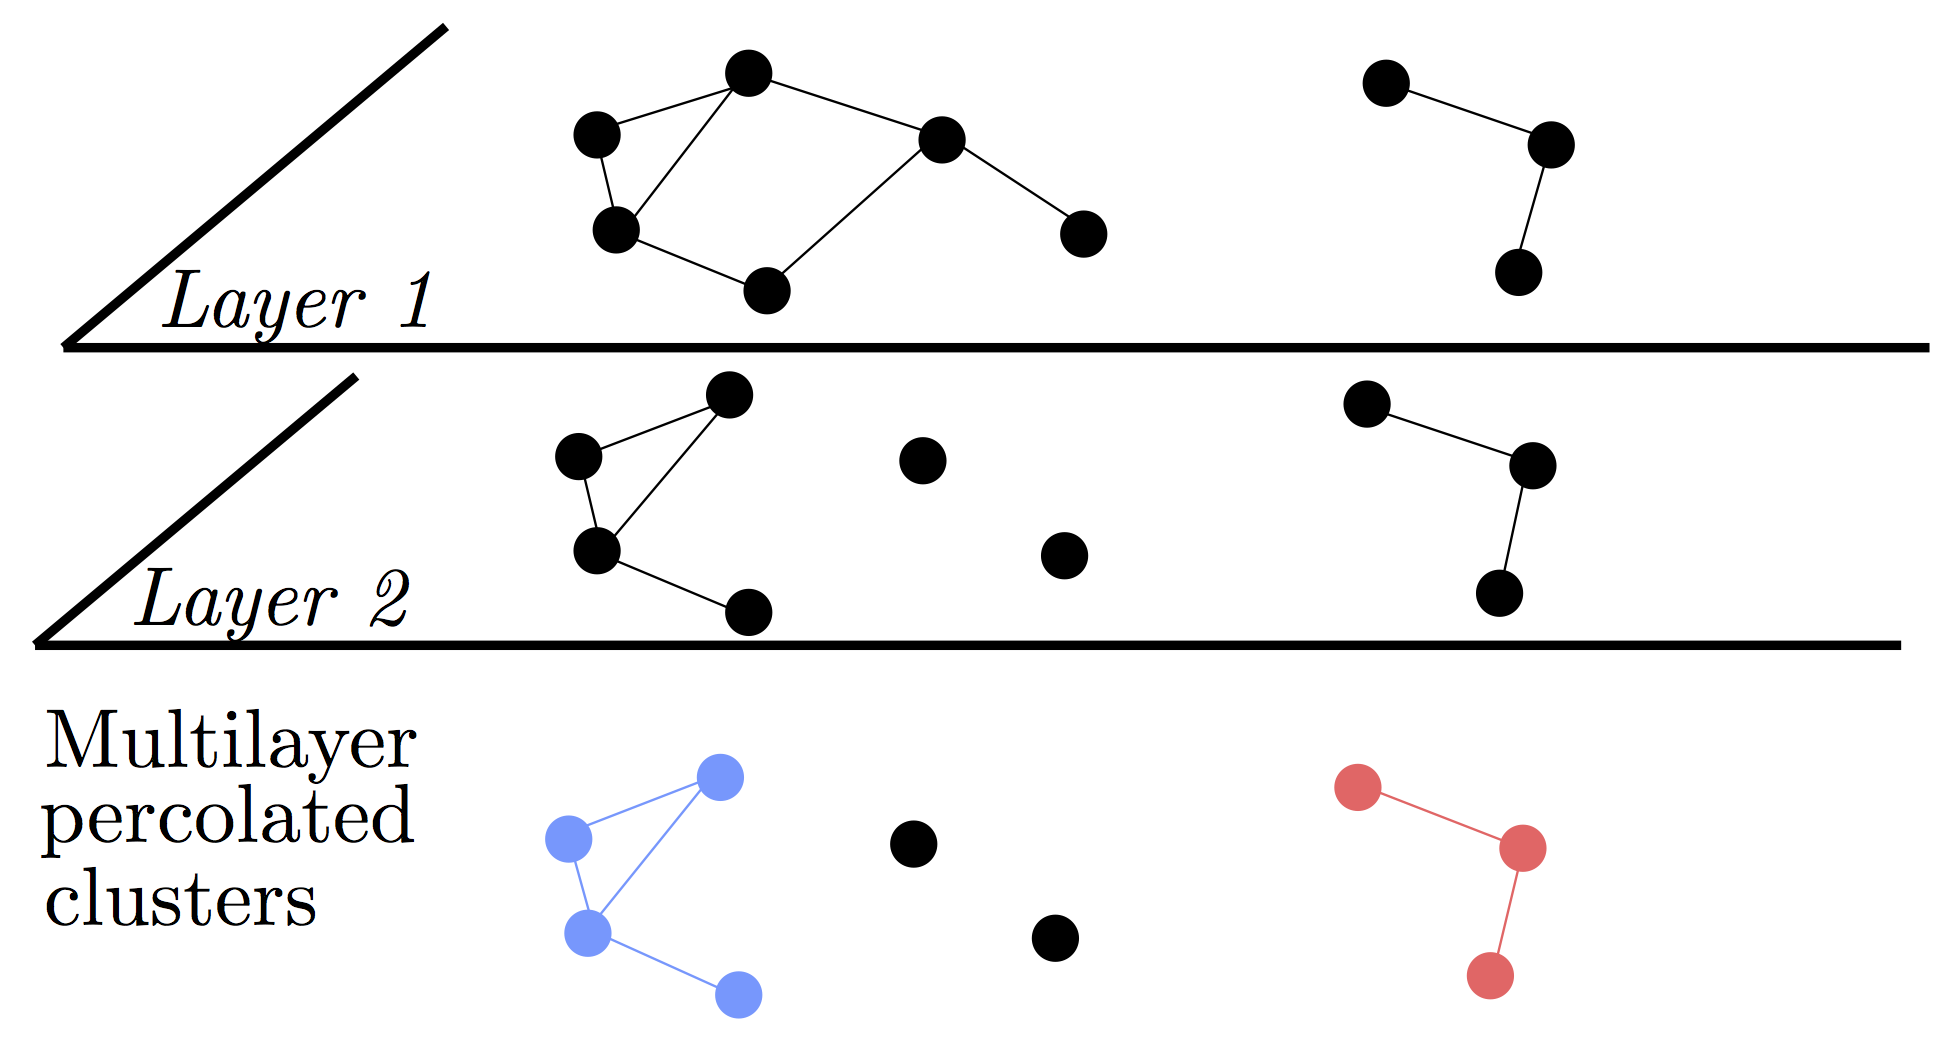
\includegraphics[width=\linewidth]{Fig1.png}}
  \centering
  \caption{Schematic representation of the multi-dimensional network percolation heuristic. Two layers are considered here, with similar nodes but different links in each. To each layer is associated a node variable. In each layer, links are created according to a distance threshold (percolation radius) and a variable value threshold. The final clusters (bottom in color) are obtained by considering the links present in each layer.\label{fig:method}}
\end{figure*}
%%%%%%%%%%%%%%%%%%%%


\subsubsection{Proposed heuristic}

Percolation processes in multilayer networks have been proposed as an extension within simple networks \citep{boccaletti2014structure}. A generalization of epidemic spreading can for example be achieved using this framework \citep{son2012percolation}. In the case of multilayer networks sharing the same nodes for all layers, often called multiplex networks \citep{aleta2018multilayer}, bond percolation has also been studied \citep{hackett2016bond}. In the case of our heuristic, bond percolation is operated between two cells given a distance threshold, and furthermore with a threshold parameter for each layer assuming a node function within each layer. The distance-based connection is similar to generative processes for random euclidian networks \citep{penrose1999k}.

We do not call our method ``multi-layer percolation'', since nodes are common between layers. We show in Fig.~\ref{fig:method} for a schematic representation of the method. It can be implemented with a propagation heuristic or directly working on adjacency matrices. The rationale behind combining a thresholding for each layer variable with a distance thresholding relies on the idea that a first component for two points to interact is a geographical proximity. The second component is a strong enough intensity of the urban dimension captured by each layer, simultaneously for all layers considered. This recalls Tobler's first law of geography \citep{tobler2004first} in a multi-dimensional way.


\subsubsection{Formal description}

More formally, let assume a set of nodes $V = v_i$ common to all layers of the network, and layers edges $E_j$ for layer $j$ taken as empty at the initial state of the algorithm. Each node has a value of the considered variables associated to each layer, written as a matrix $v_{ij}$. The algorithm works as follows:
\begin{enumerate}
	\item Percolation is first done within each layer. For each layer, a link $e_{kl} \in E_j$ is created if $d(v_k,v_l) < r_0$ where $d$ is the distance between the nodes (which can be any distance) and $r_0$ the percolation radius, and if $v_{kj} > \theta_j$ and $v_{lj} > \theta_j$ where $\theta_j$ is the threshold for layer $j$.
	\item Layers are combined, by computing the final percolated network edges $E$ as the links contained within all layers simultaneously. The multi-dimensional percolation clusters are then the connected components of this network $(V,E)$.
\end{enumerate}

 
The parameters implied in this heuristic are the percolation radius $r_0$ and the variable thresholds $\vec{\theta} = \theta_j$ for each layer $j$. Varying these parameters allows considering different levels of percolation.



\subsubsection{Application to gridded networks}

The previous generic method must be applied to a consistent urban network, in the sense of multiple variables associated to spatial nodes. To each variable then corresponds a network layer. We propose to work on gridded networks, namely nodes regularly spaced in two dimensions. In practice, these nodes will be the center of raster cells. We will consider two layers, one defined by population density and the other by road network structure indicators computed at the same resolution.



\subsection{Empirical data and network construction}


We detail now how the empirical layers were computed and the network constructed. A grid of population density morphology indicators has been computed on spatial moving windows of width 50km for all European Union by \cite{raimbault2018calibration}, with an offset resolution of 5km. From this study we get the aggregated population, producing a raster grid of population with a resolution of 5km.

Furthermore, road network topology indicators were computed at a similar resolution by \cite{raimbault2018urban}. In practice, (i) the full OpenStreetMap road network for Europe was simplified at the minimal resolution of 100m, keeping the topological properties and link attributes (including maximal speed for example); (ii) for each cell of the population morphology raster, the road network within the same spatial window of width 50km was retrieved; (iii) network structure indicators (summary statistics, centralities, etc.) were computed on this local network, providing a network indicators raster at the same resolution than population.

We use this data to construct a two layers abstract network: a layer which variable is given by population density, and a second layer which variable is given by a road network indicator. Nodes are the center of cells (thus disposed in space on a grid of step 5km). We test several possible networks by varying the road indicator taken into account for the second layer. In particular, we test the following indicators:
\begin{enumerate}
	\item number of edges $N_E$;
	\item number of vertices $N_V$;
	\item cyclomatic number $\mu$ which is defined by $\mu = N_E - N_V + c$ where $c$ is the number of connected components of the graph; this measure captures the number of distinct cycles in the graph
	\item euclidian efficiency $v_0$, defined by \cite{banos2012towards}, as the average rate between network distance and euclidian distance for all couples of links
\end{enumerate}

The choice of these measures is aimed at capturing basic aspects of network structure, and functional properties especially for the two last. Indeed, euclidian efficiency measures how the network is performant to link nodes, while the number of cycles is linked to redundancy of paths and in a way to robustness. These choice are arbitrary, but several aspects of transportation networks are still captured by these indicators. An increase of each is related to a more performant network regarding different dimensions, what is relevant for our application. A systematic study with other indicators such as centralities or accessibilities is out of the scope of this paper.



The percolation on such an abstract network is a necessary condition in our case to link the different dimensions considered, namely population distribution and local road network properties. We have therefore two levels of networks in our approach, namely the physical road network which local properties are taken here as input, and the abstract two layer network on which we do the percolation.

We will in the following write $\theta_P$ for the threshold parameter of the population layer, and $\theta_N$ for the threshold parameter of the network layer. In practice, these parameters will be given in the following as quantile level of the corresponding variable, for an easier interpretation and conception of experience plans. The name of the road network indicator considered will be written $v_N$.


%%%%%%%%%%%%%%%%
\subsection{Sustainability indicators}


As already detailed, urban regions may perform more or less well regarding different dimensions of sustainability. We propose to use the endogenous definition of regional urban systems produced by the percolation algorithm to evaluate their sustainability, in terms of conflicting objectives of economic integration and greenhouse gases emissions. The definition of sustainability, or sustainable development, is by essence multi-dimensional \citep{viguie2012trade}. Its characterization as quantitative indicators is even more subject to numerous degrees of freedom. We work here with these two stylized indicators for two conflicting dimensions, as a proof-of-concept. These dimensions can furthermore be approximated indirectly from gravity models as we will describe below. By introducing other datasets, our work could be extended to more realistic indicators and other dimensions.

We use the EDGAR database \citep{janssens2017edgar} (version 4.3.2) for local grid estimates of greenhouse gases emissions. We use the latest year available, namely 2012. As its resolution is much smaller than our indicator grid, we aggregate the emissions on the closer indicator point for each cell of the emission database. Since according to \cite{lashof1990relative} most of the greenhouse effect is caused by $\textrm{CO}_2$, and as in terms of emissions in the database we find that it represents $98.2\%$ in mass proportion of all gases, we only consider it.

Applying a gravity model to each region, we estimate abstract transportation flows within each with a gravity model. More precisely, following \cite{raimbault2018indirect}, a potential flow between two points $i$ and $j$ can be estimated with the following expression 

\begin{equation}
\phi_{ij}^{(k)} = \left(\frac{v^{(k)}_i v^{(k)}_j}{(\sum_l v_l)^2}\right)^\gamma \cdot \exp\left(\frac{-d_{ij}}{d_0}\right)
\end{equation}

where $v^{(k)}_i$ are either population or effective local GHG emissions computed with the EDGAR database (indexed by $k = 1,2$ respectively), $d_{ij}$ the distance between the two points, $d_0$ a distance decay parameter, and $\gamma$ a scaling parameter. Indeed, the economic activity follows relatively well scaling laws of populations \citep{bettencourt2007growth}, the exponent being dependant on the activity and the definition of areas on which it is estimated~\citep{cottineau2017diverse}. The distance decay captures the geographical span of potential interactions. These two parameters $\gamma,d_0$ are left free and varying them allows considering stylized configurations, such as long or short span interactions, or infra- or supra-linear scaling activities. Finally, considering the flow with the population variable ($k=1$) provides a proxy for economic flows, while with the GHG emissions ($k=2$) it provides a proxy for emissions in relation with this economic activity. Indeed, effective emissions are linked to local emissions and transportation emissions linked to the intensity of flows.

We then consider the sum of all these flows of points within the geographical span of a given cluster of nodes in our network. These clusters are obtained with the percolation method described above, and are numbered by $1 \leq c \leq C$. For the sake of simplicity, we approximate the corresponding geographical area as the convex Hull envelope of the points in the cluster, that we write $K_c$. By cumulating the flows, we therefore define the total economic flow as the sum of economic flows by 

\begin{equation}
E_c = \sum_{i,j \in K_c} \phi_{ij}^{(1)}
\end{equation}

and the total emissions due to flows by

\begin{equation}
G_c = \sum_{i,j \in C_c} \phi_{ij}^{(2)}
\end{equation}

These indicators have no interpretable unit and need to be renormalized. This allows defining a relative economic inefficiency by 

\begin{equation}
e_c = 1 - \frac{\max_c E_c - E_c}{\max_c E_c - \min_c E_c}
\end{equation}

where $\max_c E_c$ (resp. $\min_c E_c$) is the maximal (resp. minimal) value of $E_c$ across all clusters. We define in a similar way the relative potential emissions by

\begin{equation}
g_c = \frac{\max_c G_c - G_c}{\max_c G_c - \min_c G_c}
\end{equation}

where $\max_c G_c$ (resp. $\min_c G_c$) is the maximal (resp. minimal) value of $G_c$ across all clusters.

Both indicators should be minimized for sustainability. Their value is dependant on the number of clusters and their extent, i.e. the geographical surface they cover. To be able to compare values across different clusterings (corresponding to different parameter values for the percolation heuristic), we finally define normalized indicators $\tilde{e}_c,\tilde{g}_c$ in a similar way, but the extrema being computed on all other possible urban configurations with the same $\gamma,d_0$ values.

Using these potential flows follows the logic of \cite{arbabi2019development} which shows a need for improved intra-city-region mobility in England and Wales. Considering the regions as entities in which such transportation development policies can more easily been developed, we look at the sustainability of different possible regions if these potential flows were realized. Varying the parameters $\gamma$ and $d_0$ allows to control for the economic activity considered (high $\gamma$ values correspond to high added-value activities) and the span of interactions through $d_0$.

For descriptive purposes, we also consider summary measures of clusters, as the population $P_c$ and effective emissions $EM_c$ taken as the sum of population (resp. emissions) of the points in $K_c$.


\section{Results}

\subsection{Implementation}


In practice, the analysis is implemented using R and the igraph package. Source code, data and results are available on the open git repository of the project at \url{https://github.com/JusteRaimbault/UrbanMorphology}. The network is constructed by superposing the population density layer with the network layer, starting from the 5km resolution spatial fields for morphological and network indicators. This network is filtered with the threshold parameters for each layer and with the radius parameter. Connected components yield the clusters that we interpret as endogenous regions.



%%%%%%%%%%%%%%%%%%%%
\begin{figure*}[ht] 
%\resizebox{10cm}{7cm}
  {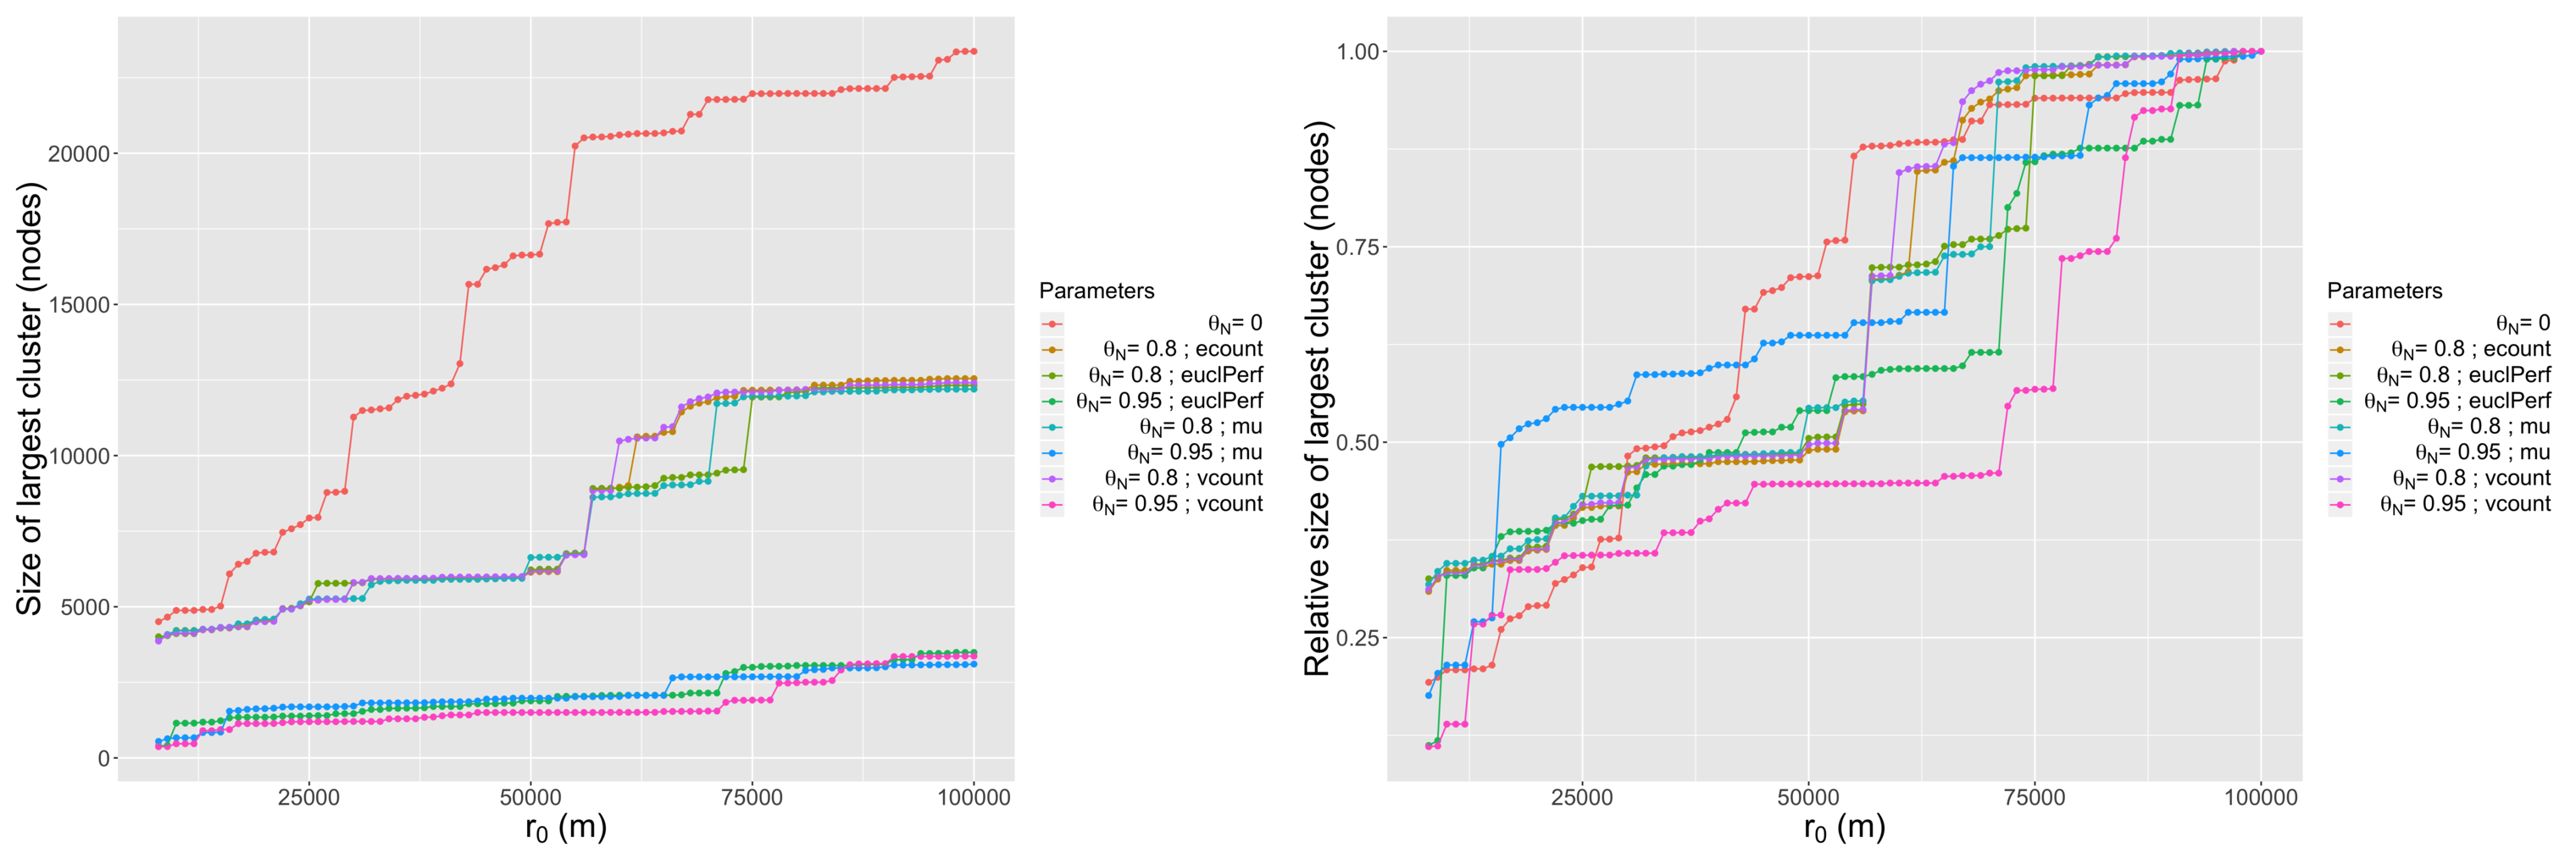
\includegraphics[width=\linewidth]{Fig2.png}}
  \centering
  \caption{Percolation transition. On the left, we plot the size of the largest cluster in each configuration in terms of nodes, as a function of the percolation radius $r_0$. Color gives the other percolation parameters. On the right, the plot is similar but with the size relative to the size of the largest cluster obtained with the maximal radius in each configuration.\label{fig:percolation}}
\end{figure*}
%%%%%%%%%%%%%%%%%%%%

%%%%%%%%%%%%%%%%%%%%
\begin{figure*}[ht] 
%\resizebox{10cm}{7cm}
  {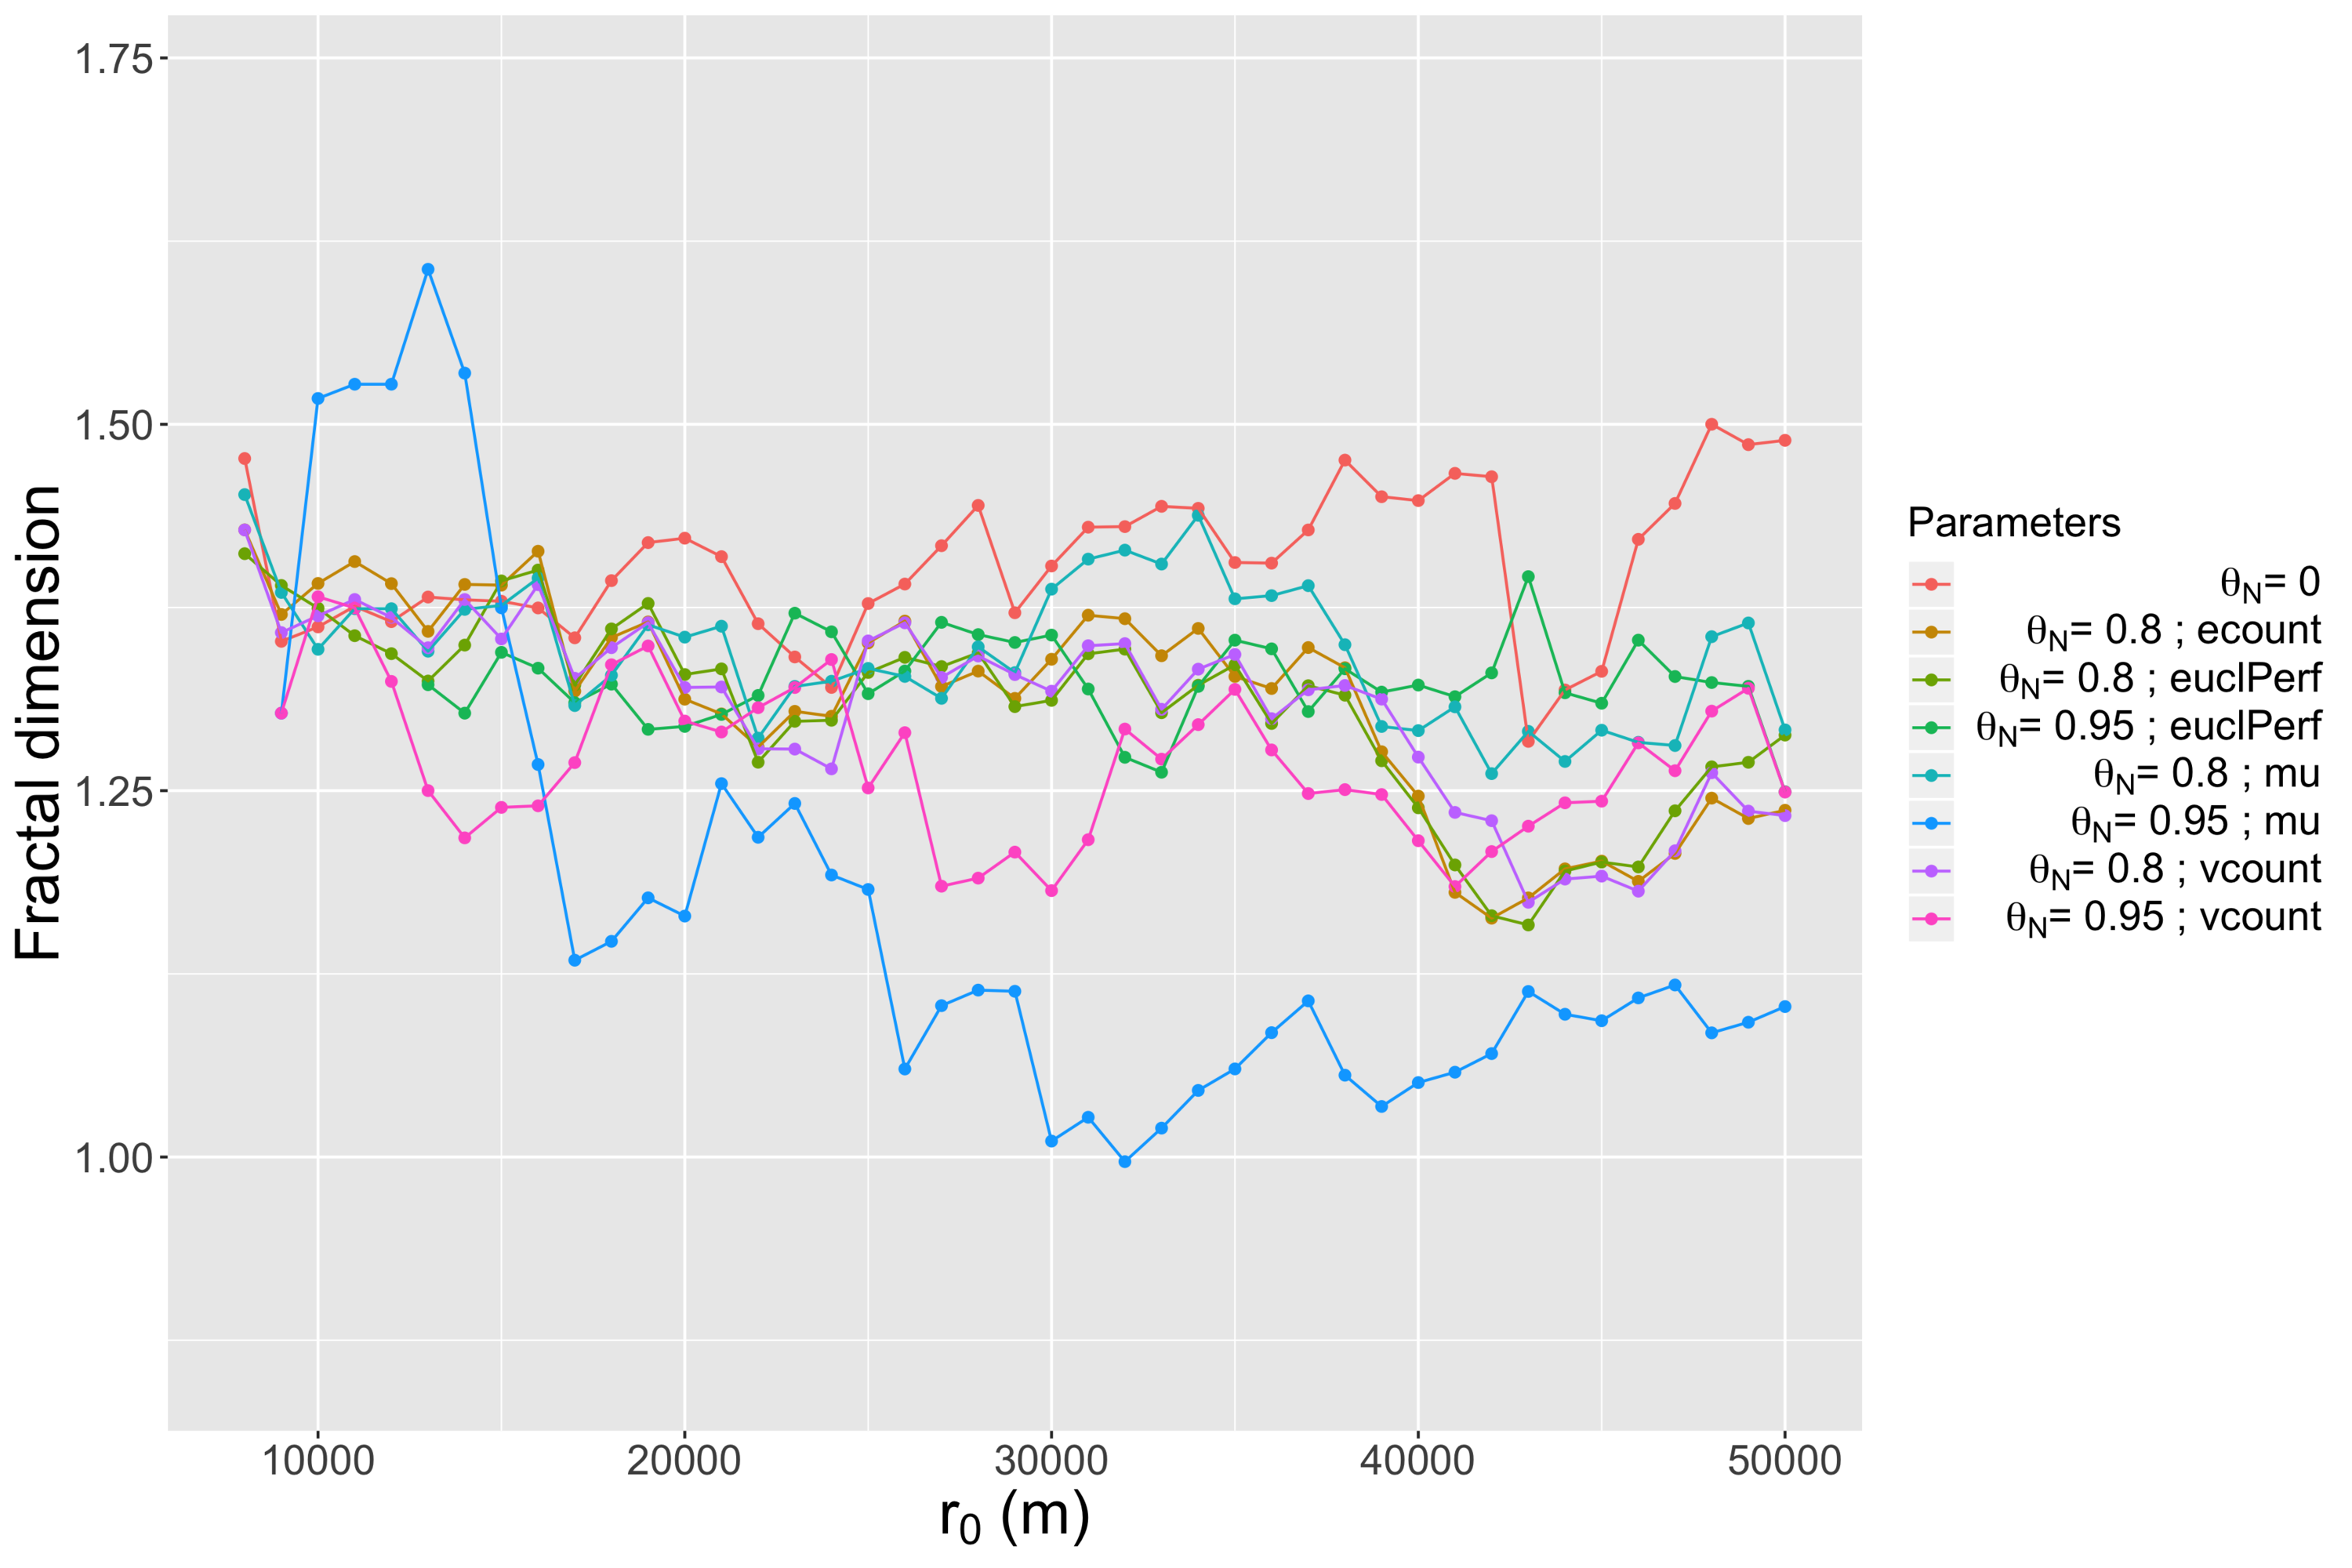
\includegraphics[width=\linewidth]{Fig3.png}}
  \centering
  \caption{Fractal dimension. We plot for each parametrization given by the curve color the evolution of the fractal dimension $\alpha$ as a function of $r_0$. Standard errors are not plotted for readability.\label{fig:fractaldim}}
\end{figure*}
%%%%%%%%%%%%%%%%%%%%

%%%%%%%%%%%%%%%%%%%
\subsection{Percolation transition and fractal dimension}



In its application to road networks by \cite{arcaute2016cities}, the structure of the national urban system for UK is captured by studying the percolation transition, i.e. the variation of the size of the largest cluster as a function of the percolation radius. As this signature is tightly linked to historical, cultural and geographical conditions, the application to different urban systems should yield different results. We study here this property, for different threshold parameter values. We make the radius vary between 8km and 100km with a one km step, have a fixed population threshold $\theta_P = 0.85$, test all road network indicators, and three network layer thresholds $\theta_N \in \{ 0 ; 0.8 ; 0.95 \}$. These values yield a good precision for the radius which is the most important variable to study transition and estimate fractal dimensions, while this population threshold is enough to provide a broad coverage for large radiuses (as shown by other explorations described below). Changing network variables and their threshold allows us to investigate how the transition behavior do change regarding the dimension considered and its intensity.

The absolute and relative sizes of the largest cluster are plotted in Fig.~\ref{fig:percolation} as a function of the percolation radius. This aspect first gives methodological information on multilayer percolation. Indeed, comparing the result with $\theta_N = 0$ (single layer percolation) with positive values of $\theta_N$ shows a significantly different behavior. As expected, absolute size are much smaller, but when looking at relative sizes we observe that the abrupt steps typical to percolation transitions have different distributions across the different parametrizations. This result is particularly interesting regarding the first axis of our research question, as it shows that the structure of clusters obtained is not only due to the population layer, and that the multi-dimensional percolation captures a complementary signal.
 
The more regular curve seems to be the standard percolation on population only, whereas at $\theta_N = 0.95$, different road network indicators produce either very early transitions (for $\mu$ for example) or very late (for $N_V$). Also, changing of scale compared to \cite{arcaute2016cities} gives more steps and less abrupts curves in general, confirming the integration of subsystems with different structures in our analysis and the importance of scale in such analysis. As the addition of a layer also changes drastically the results, one should stay careful when switching from a mono-dimensional percolation to a multi-dimensional percolation.


We study also the evolution of the fractal dimension of clusters as a function of $r_0$, to verify how the initial percolation approach is robust to multi-dimensionality. Following \cite{arcaute2016cities}, we estimate the fractal dimension $\alpha$ of clusters with a simple OLS regression between cluster size and cluster diameter, namely 

\begin{equation}
\log N_c = k + \alpha \cdot \log \delta_c
\end{equation}

where $N_c$ is the size of cluster $c$ and $\delta_c$ its diameter. These estimations are shown in Fig.~\ref{fig:fractaldim}. As a negative result, which could be due to the abstract nature of our network, a clear maximum in the value of the fractal dimension can not be found. Either it is located at a resolution that our method can not reach due to the minimal 5km limit imposed by the abstraction in the network construction, or it does not exist when coupling dimensions. Determining which assumption is more plausible is out of the scope of this paper.

We do not plot the standard error $\sigma$ of fractal dimensions (obtained as the estimation error in the OLS) for visibility purposes, but their relative value given by $\alpha / \sigma\left[\alpha\right]$ is in average 0.10 and in maximum 0.196 on all points, meaning that these estimations remain however consistent.

Regarding the variability of fractal dimension as a function of the percolation radius $r_0$, we study the possible existence of a significant maximum when $r_0$ varies. We therefore simply consider the difference $(\alpha - \sigma\left[\alpha\right])_M - (\alpha - \sigma\left[\alpha\right])_m$ where the first is taken at the maximum value of $\alpha$ and the other at its minimum value. This intuitively corresponds to checking if confidence intervals do not overlap between the maximum and the minimum of the curve. We find that the configuration for $\mu$ and $\theta_N=0.95$ has a clearly significant maximum (difference at 0.38). For this coupling, the endogenous structure given by the maximum may be defined. Other configurations yield non-significant maximums (negative values of the difference).


This study of percolation transition and fractal dimension thus shows that our multi-dimensional percolation heuristic remains relevant, as results analog but qualitatively different to the one-dimensional approach can be obtained.


%%%%%%%%%%%%%%%%%%%%
\begin{figure}[h!] 
%\resizebox{10cm}{7cm}
{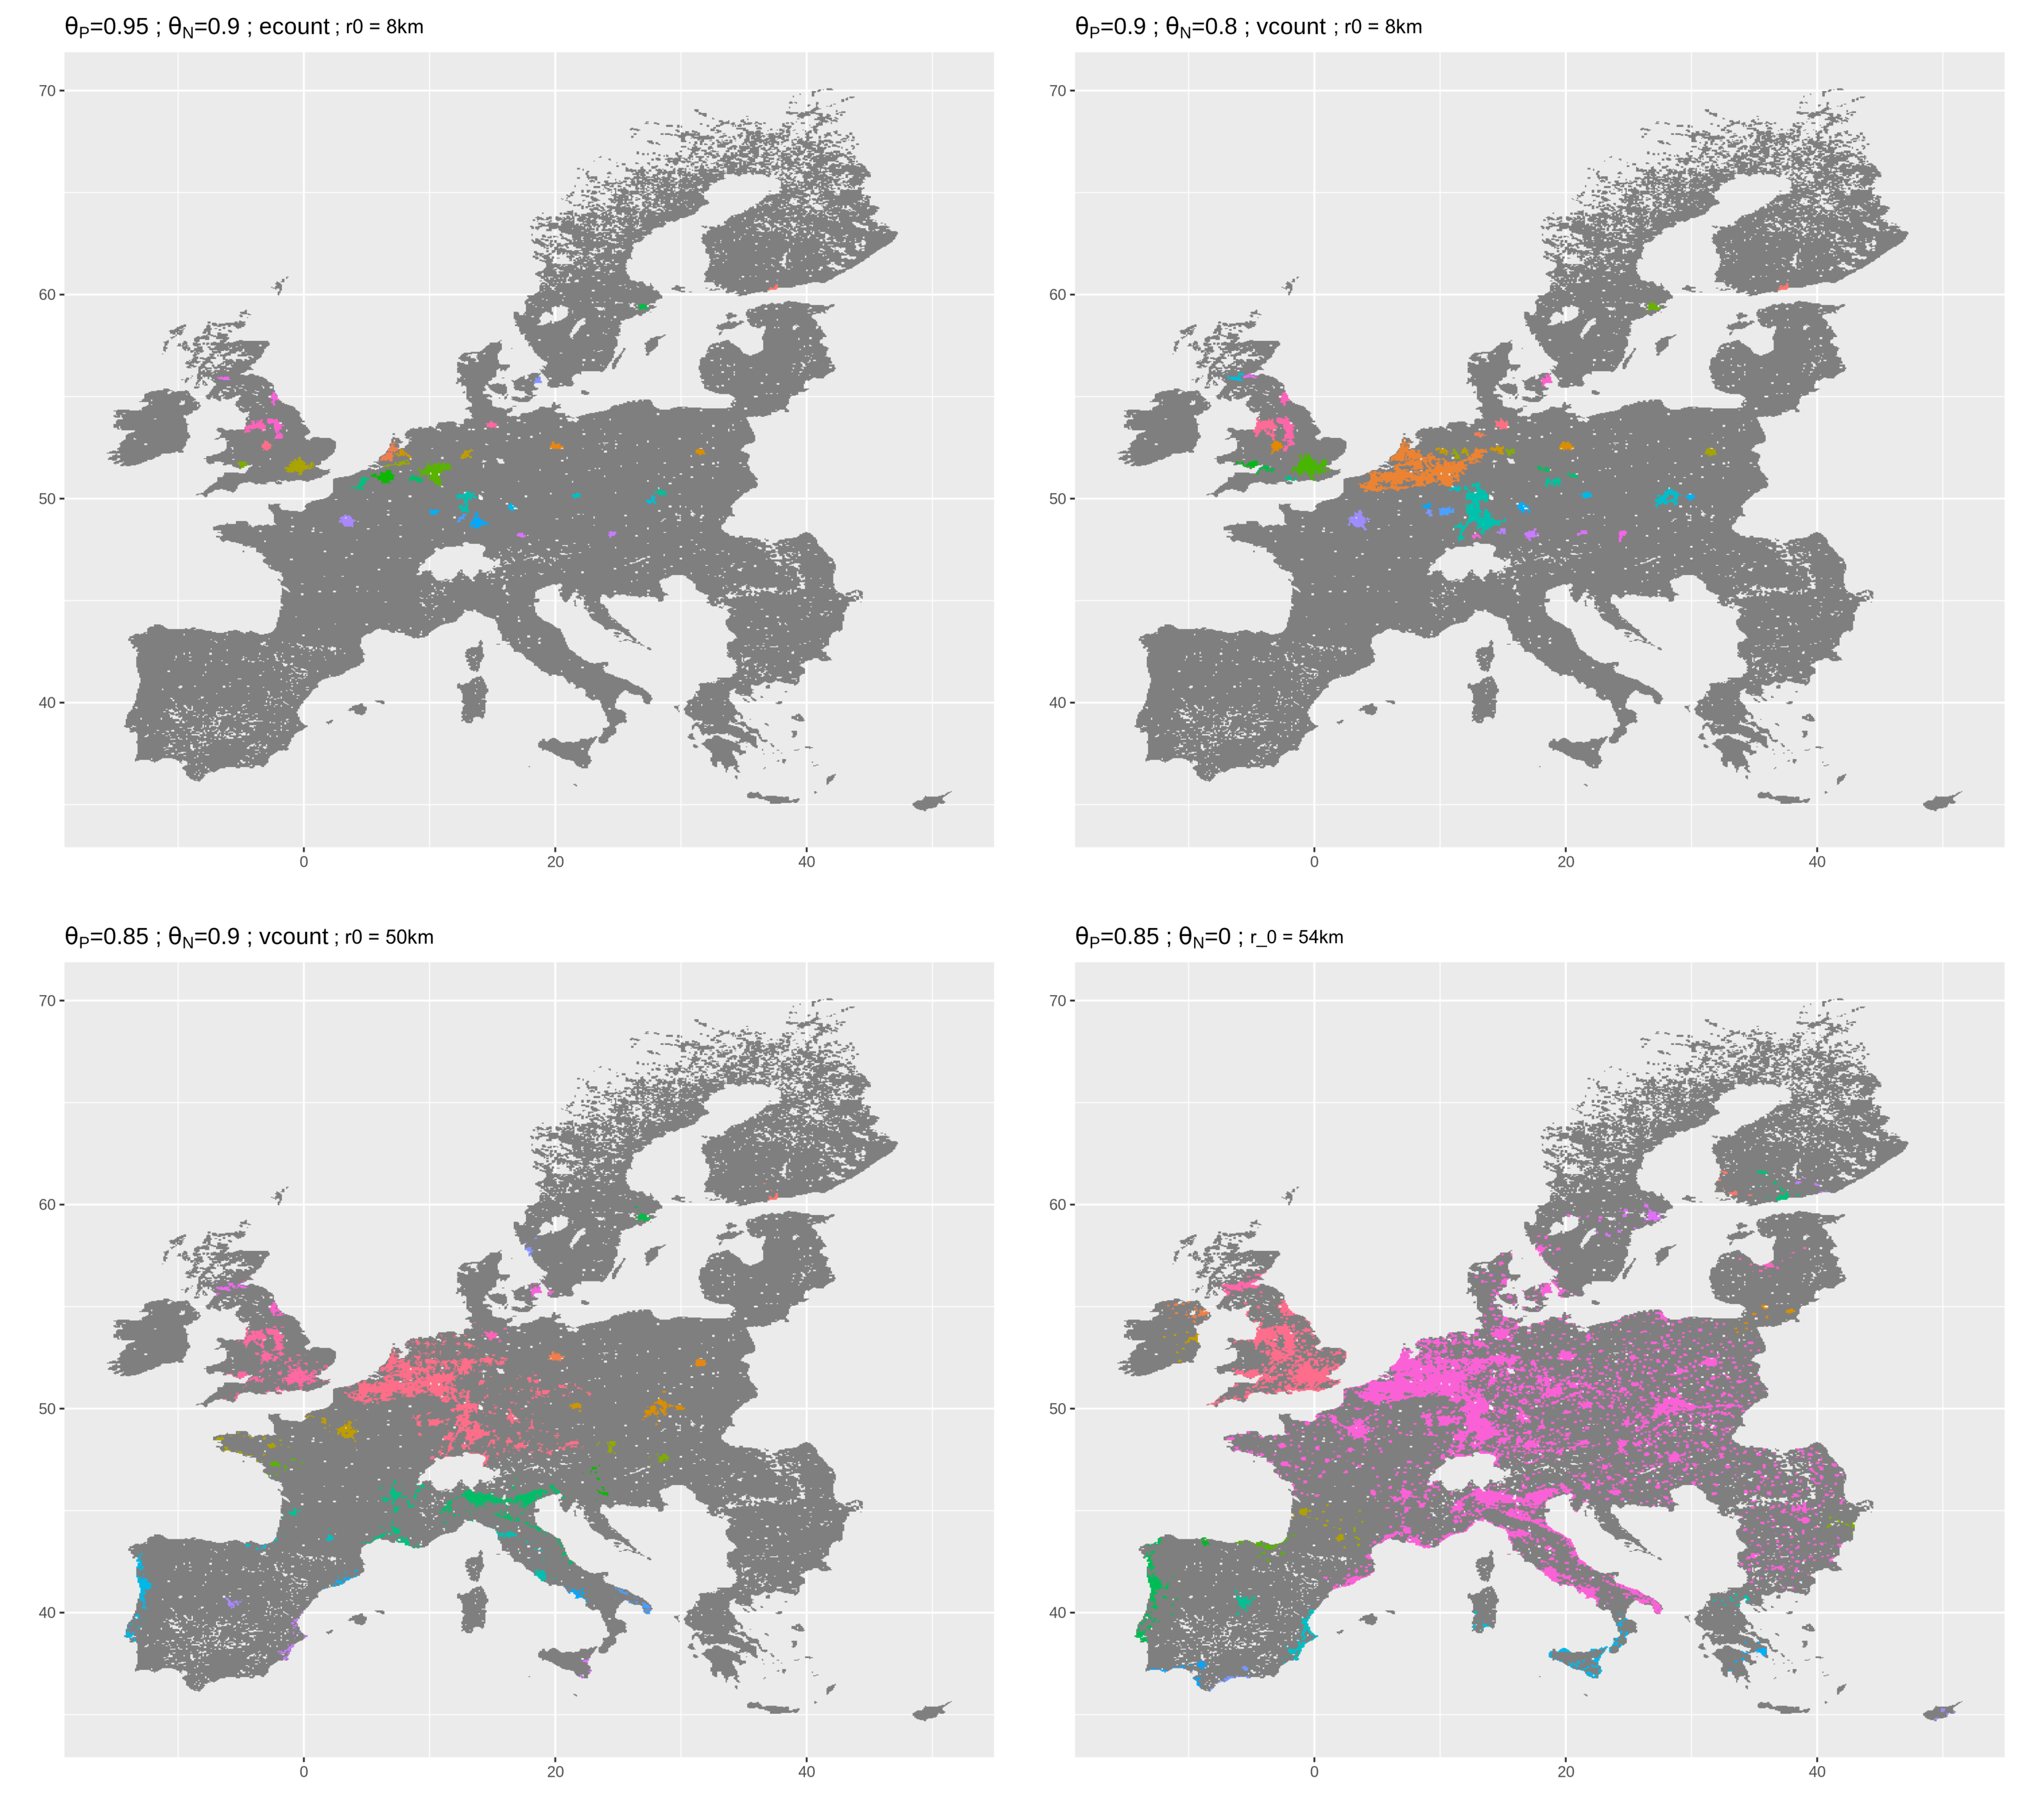
\includegraphics[width=\linewidth]{Fig4.png}}
  \centering
  \caption{Examples of obtained clusters for different parameter values. In the top-right case for example ($\theta_P = 0.9$, $\theta_N = 0.8$, variable \texttt{vcount},$r_0 = 8km$), we obtain the urban regions of West midlands and London in the UK, Randstad merged with Rhein-Rhur and Rhein-Main in Germany, Paris in France, also with capital cities such as Copenhaguen, Stockholm and Helsinki. There is no cluster in South Europe in that case, due to the high population density threshold.\label{fig:exclusters}}
\end{figure}
%%%%%%%%%%%%%%%%%%%%


%%%%%%%%%%%%%%%%%%%%
\begin{figure}[h!] 
%\resizebox{10cm}{7cm}
  {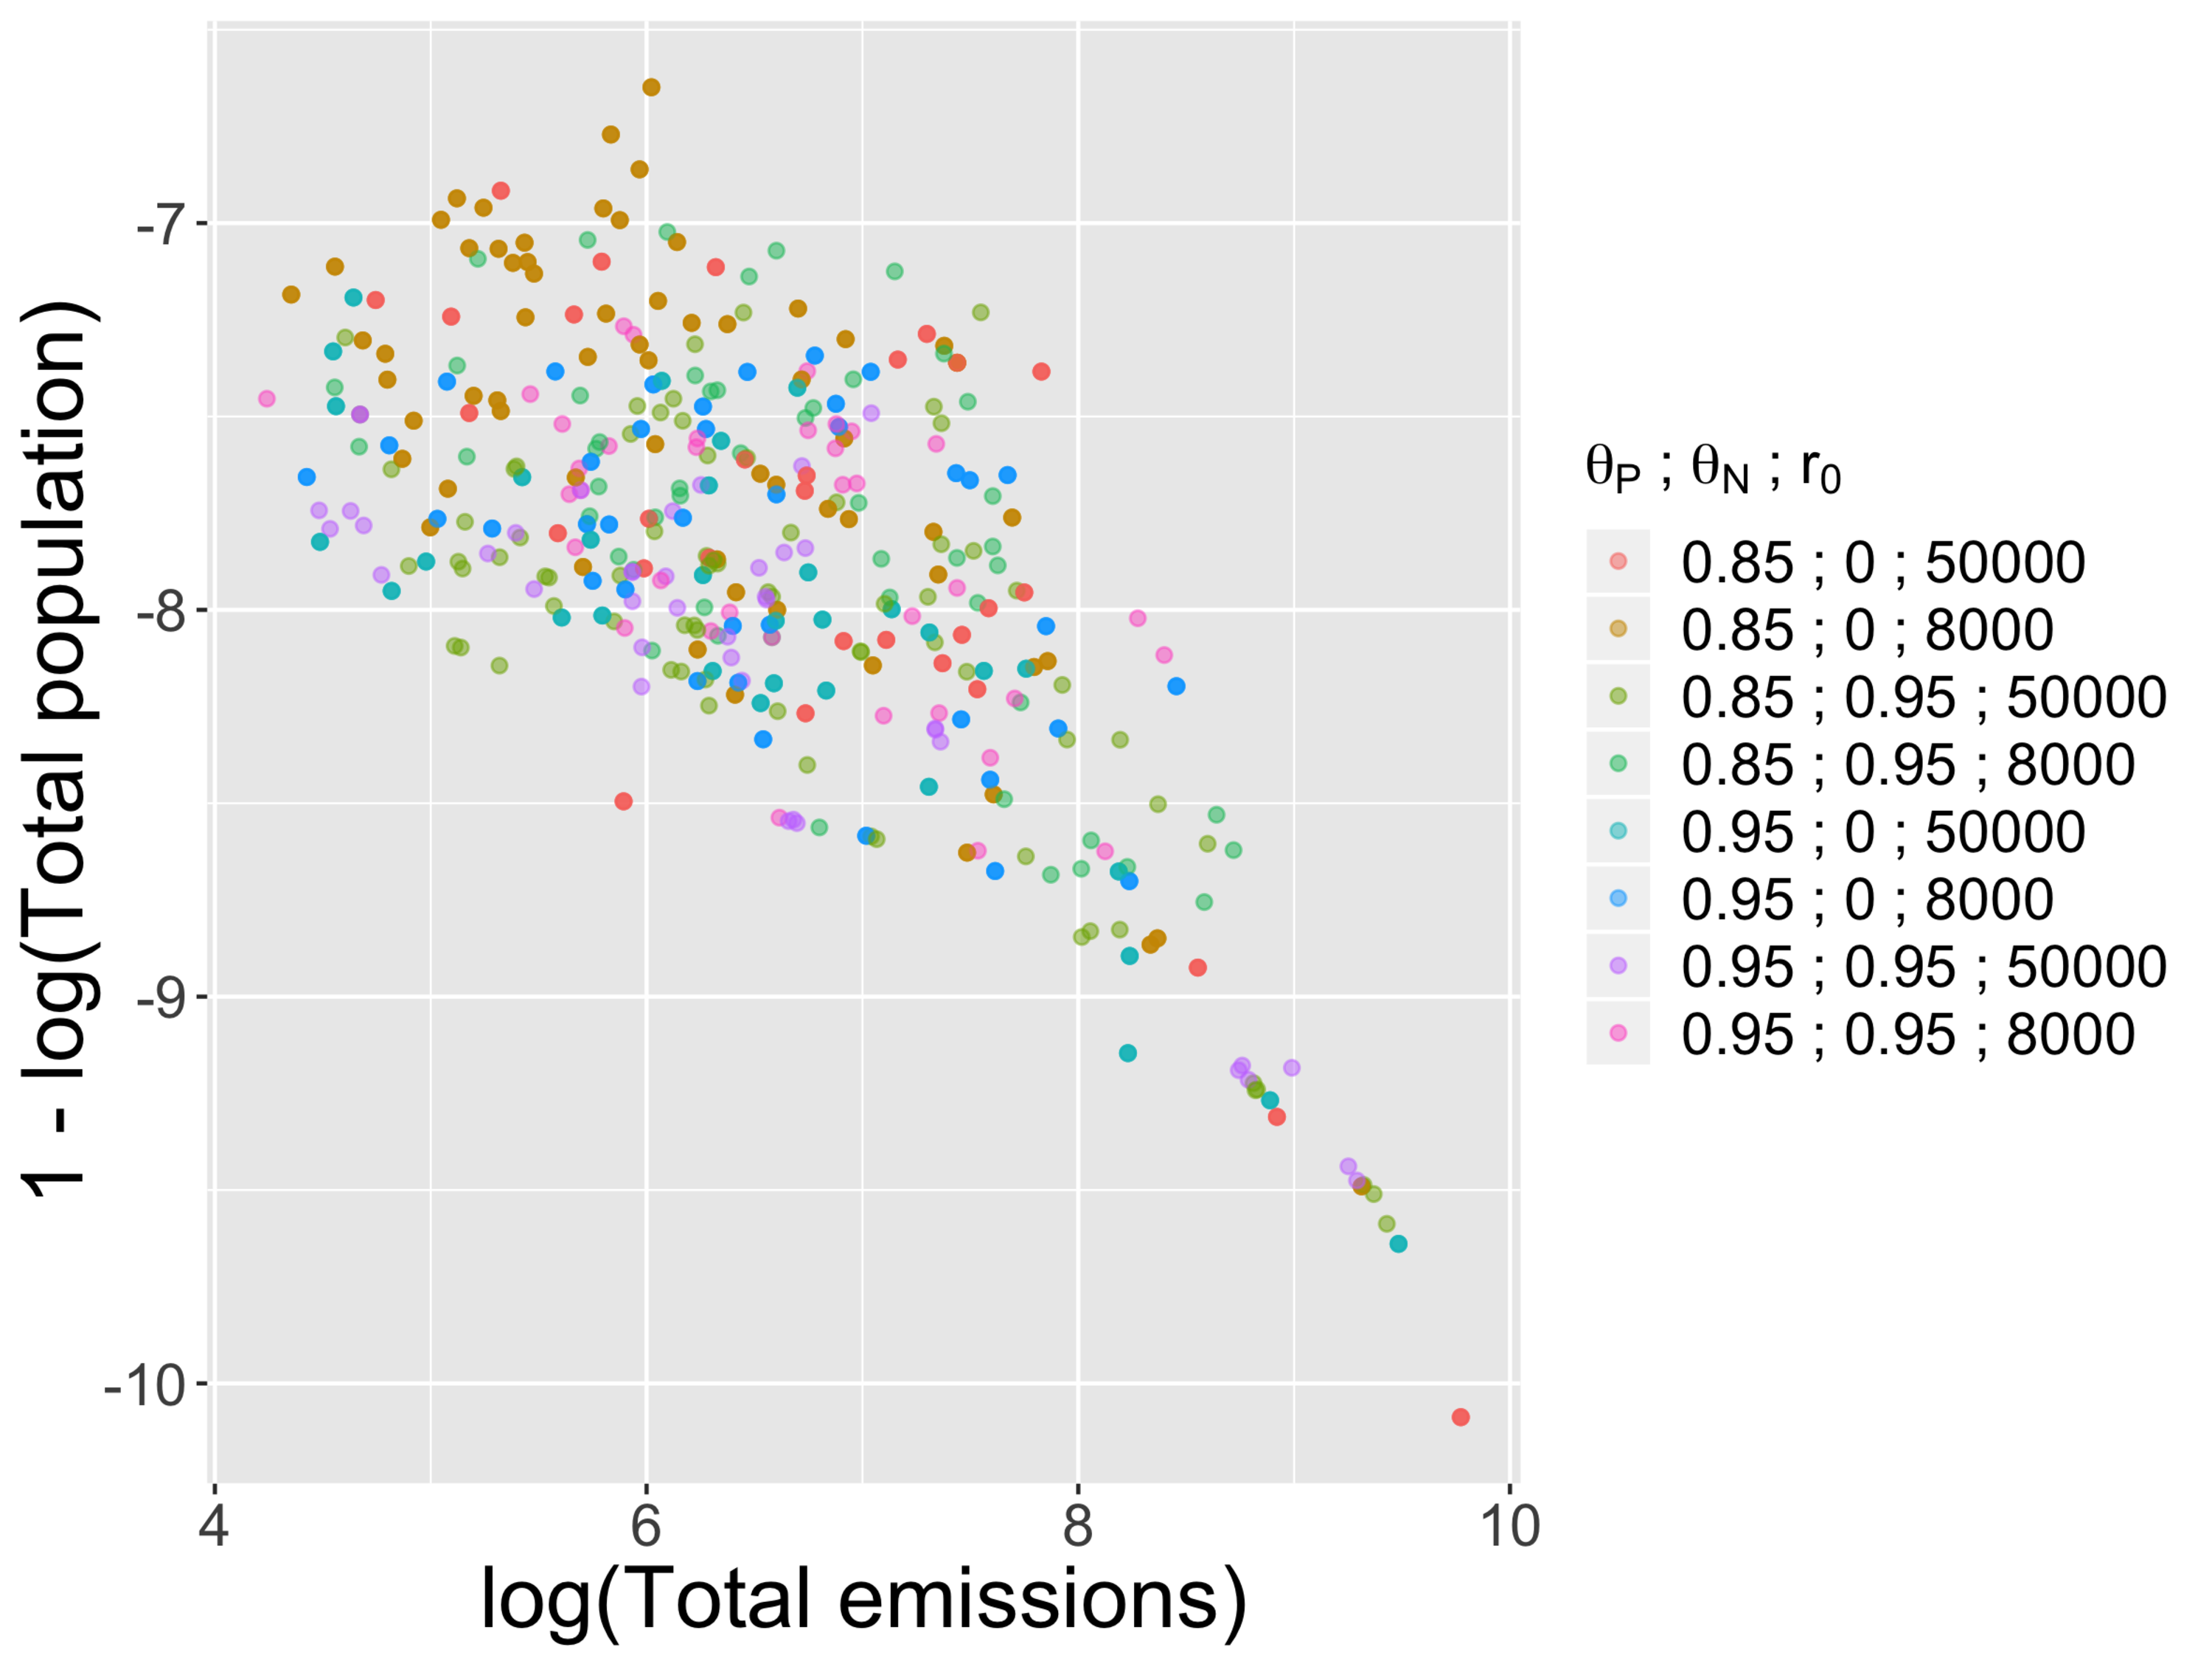
\includegraphics[width=0.7\linewidth]{Fig5.png}}
  \centering
  \caption{Point clouds of region-level indicators, namely population and emissions, for different parametrizations, given by the color. Each point represent an endogenous urban region.\label{fig:paretos}}
\end{figure}
%%%%%%%%%%%%%%%%%%%%

%%%%%%%%%%%%%%%%%%%%
\subsection{Extracting endogenous mega-city regions}


We now switch the experience plan to a full grid, for parameters $r_0$, $\theta_P$, $\theta_N$ and the road network indicator considered, and also make $\gamma$ and $d_0$ vary. We systematically explore the clusters obtained for 4800 parameter configurations, such that for all road network indicator, $\theta_P \in \{ 0.8 ; 0.9 ; 0.95 \}$, $\theta_N \in \{0 ; 0.8 ; 0.95 \}$, $r_0 \in \{ 8 ; 10 ; 15 ; 20 ; 50\}$ km, $\gamma \in \{ 0.5 ; 1 ; 1.5 ; 2\}$, and $d_0 \in \{ 0.1 ; 1 ; 10 ; 50 ; 100\}$ km.


We obtain very different endogenous morphologies for the different parametrizations. Maps reveal that some configurations resemble the actual distribution of European mega-city regions, which are functionally integrated polycentric urban areas \citep{hall2006polycentric}. These are here defined endogenously from the bottom-up and have a priori no reason to coincide with these functional regions. We show some examples in Fig.~\ref{fig:exclusters}. The first map of this figure, obtained for high population and network thresholds ($\theta_P = 0.95$ and $\theta_N = 0.9$), but a low radius $r_0 = 8$km and edge count $N_E$ to define the road network layer, include several mega-city regions described by \citep{hall2006polycentric}, namely London metropolitan area, the Randstad in Netherland, the Rhein-Main and Rhein-Ruhr in Germany, Greater Paris in France, Brussels area in Belgium. The same parameters with $\theta_N = 0$ yield not exactly the same regions, as confirmed by the transition curves in Fig.~\ref{fig:percolation}, what means that our approach taking into account two dimensions may capture effective processes of mega-city regions, in particular by including the road network which is crucial as these regions are integrated in terms of flows. The bottom-left map show an example of large clusters emerging in UK and in the center of Europe, the South remaining largely disconnected. Finally, the last map shows the result obtained with a very high radius $r_0 = 54$km, with a giant cluster spanning most of Europe. UK is still disconnected and the transition where it connects happens at $r_0 = 55$km. This does not necessarily mean that UK should be disconnected from continental Europe, as we considered geographic distances only, hiding the high speed connection of the Channel tunnel.


The behavior of sustainability indicators for different population, network and distance thresholds yield different distributions of performances across clusters within a configuration but also between configurations. Before considering the flow-based indicators described above, we can already study basic summary measures such as population $P_c$ and effective emissions $EM_c$. We show in Fig.~\ref{fig:paretos} point clouds of $\log EM_c$ against $1 - \log P_c$ for some configurations. Indeed, regarding the population it contains, an area can be more or less efficient in terms of emissions. Seeing the population as an objective to be maximized (thus the plotted value to be minimized) while the emissions must be minimized, we observe a Pareto front for all points (i.e. all clusters across all configurations). Given different dimensions to be minimized, a Pareto front consists of the points which are not Pareto-dominated by any other point, i.e. that there exists no other point performing best on all objectives. In practice, this yields optimization compromises in the context of multi-objective optimization, when no aggregation of the dimensions is possible or desirable. In Fig.~\ref{fig:paretos}, the front is the lower bound of the point cloud. We also find no dominating point for each configuration, i.e. that considering point clouds of a single color, a Pareto front with more than one point is still present. Some clusters are therefore optimal compromises in the Pareto sense in each configuration, while some are dominated and thus not efficient. This confirms that urban systems are generally compromises between multiple objectives.


%%%%%%%%%%%%%%%%%%%%
\begin{figure*}[!ht] 
%\resizebox{10cm}{7cm}
  {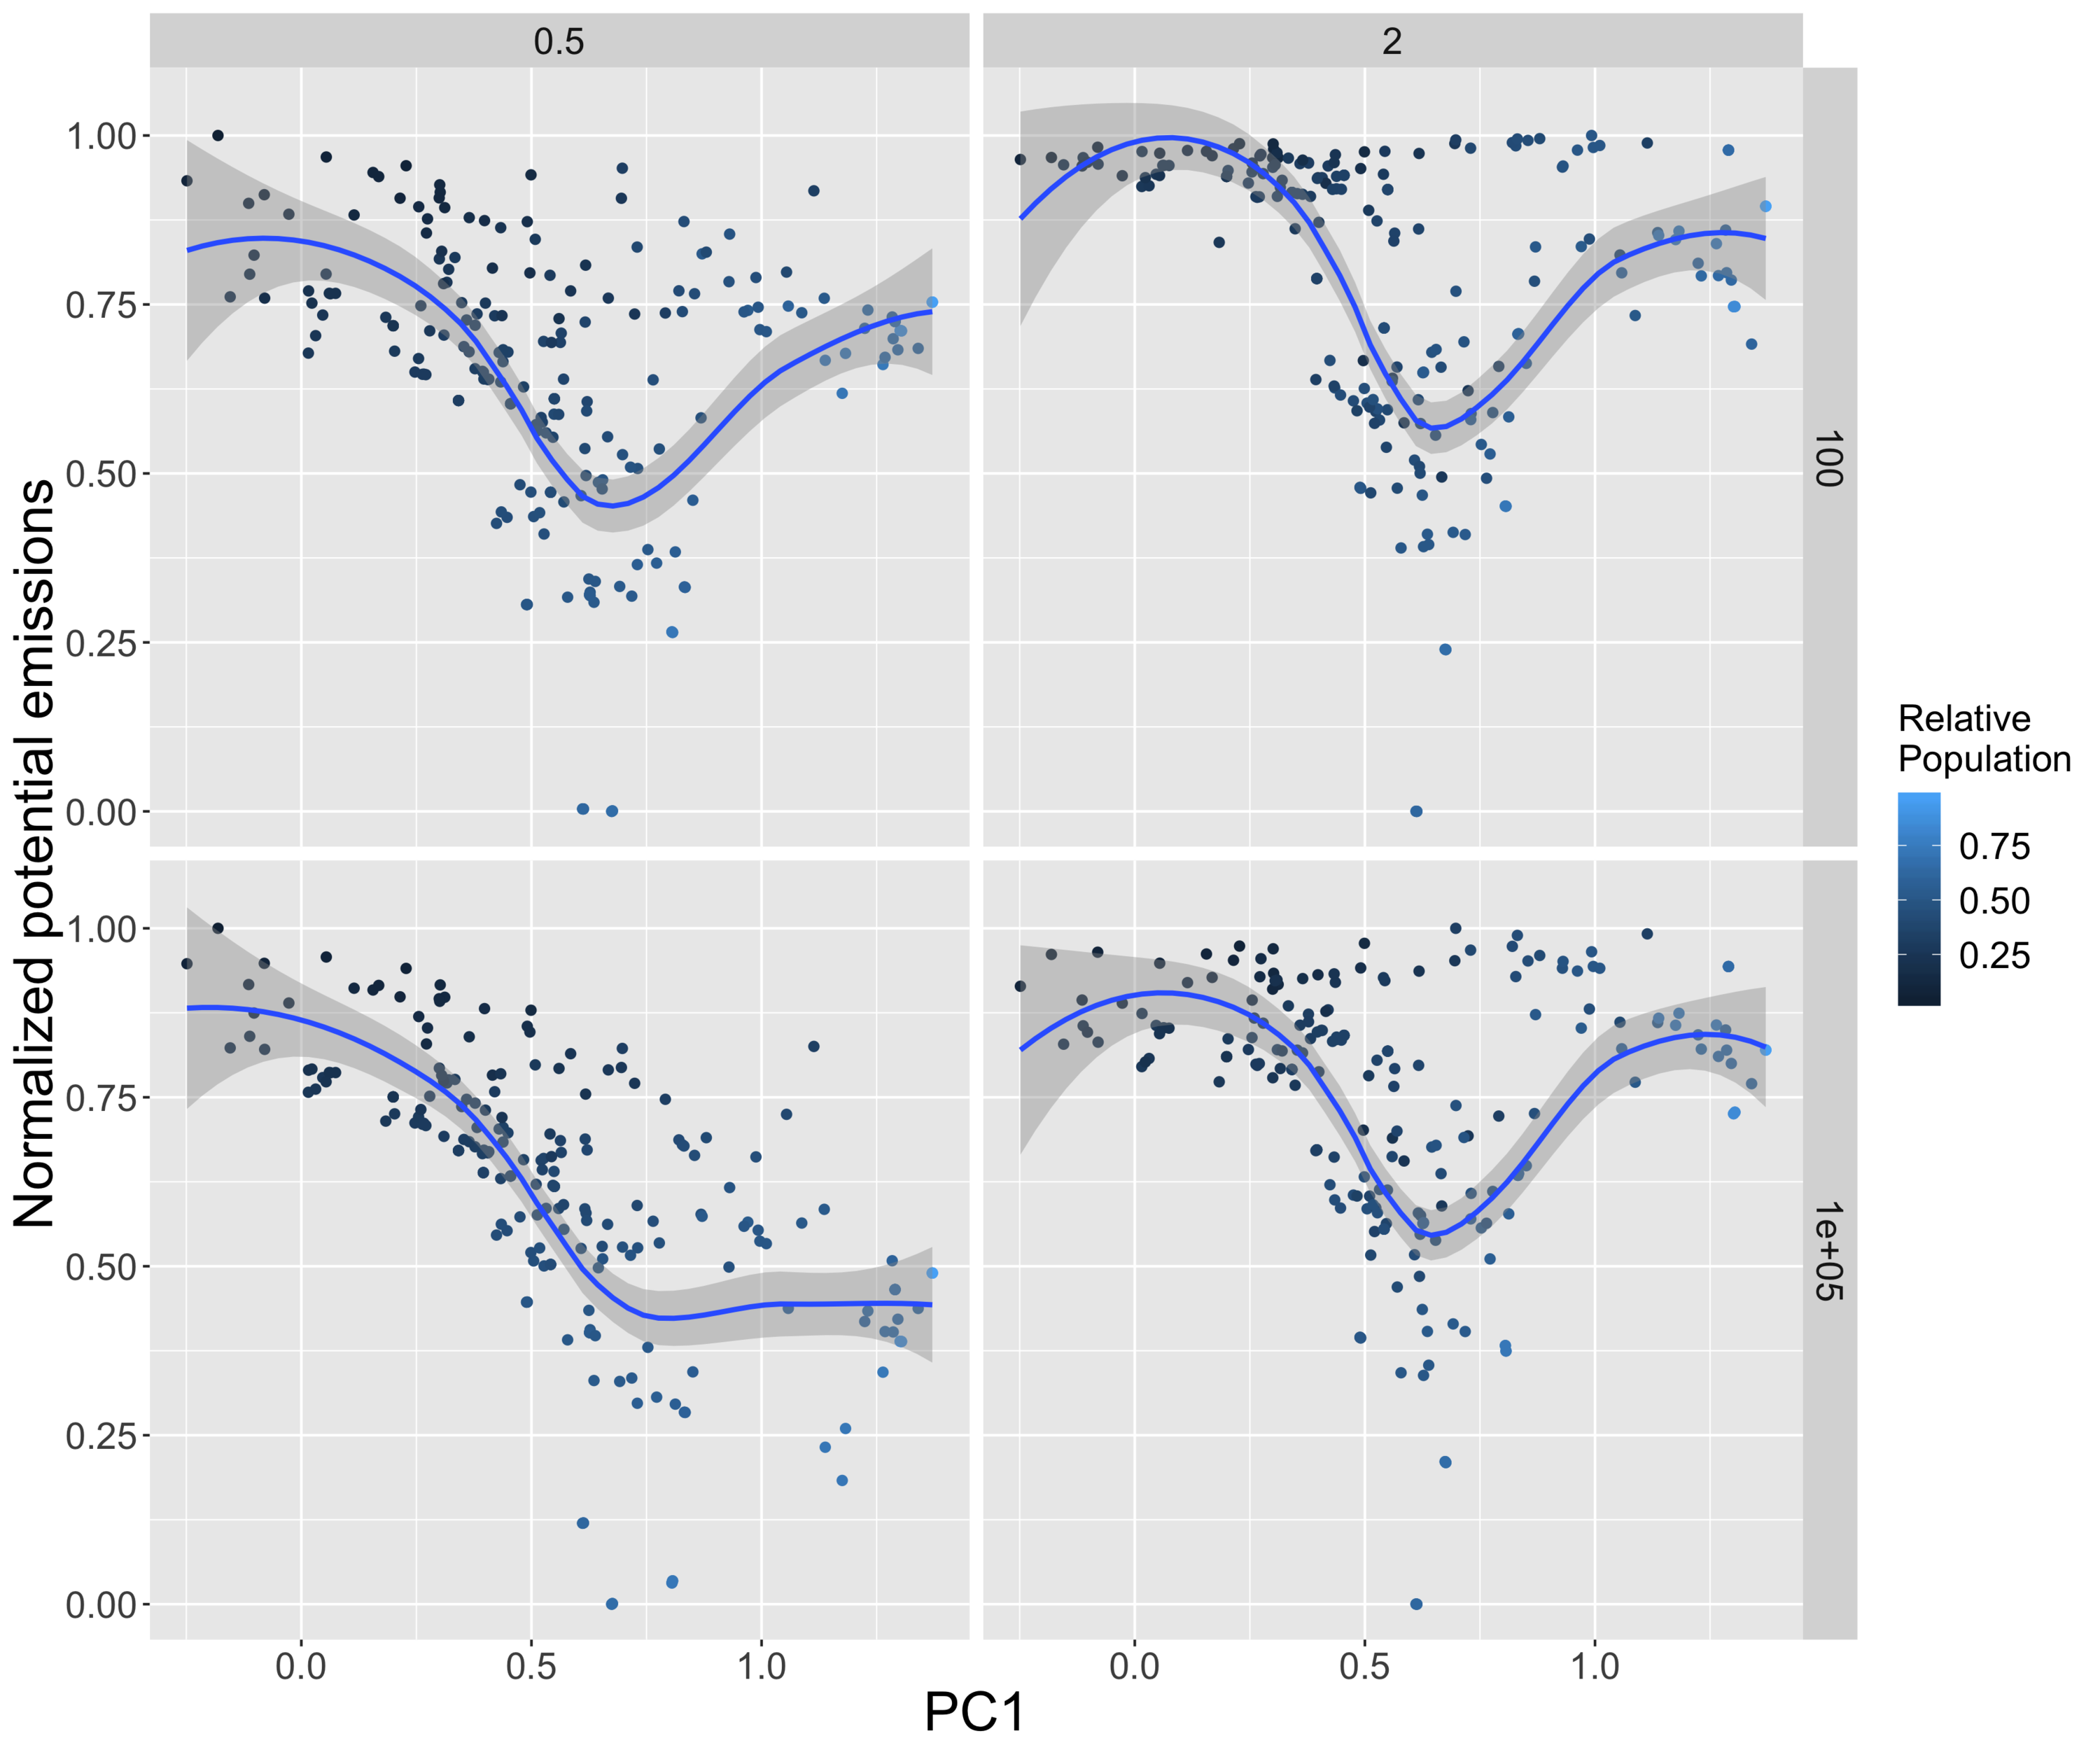
\includegraphics[width=\linewidth]{Fig6.png}}
  \centering
  \caption{Aggregated values of normalized potential emissions $\sum_c \tilde{g}_c$, as a function of the first morphological principal component (PC1), for varying values of parameters $d_G$ (rows) and $\gamma_G$ (columns). Other intermediate values for these parameters yield similar behaviors. As PC1 is mainly linked to monocentricity, there seems to exist an optimal intermediate level of monocentricity for emissions alone. Color level give the share of population within the considered clusters in comparison to all European population.\label{fig:emissions-pc1}}
\end{figure*}
%%%%%%%%%%%%%%%%%%%%


%%%%%%%%%%%%%%%%%%%%
\begin{figure*}[!ht] 
%\resizebox{10cm}{7cm}
  {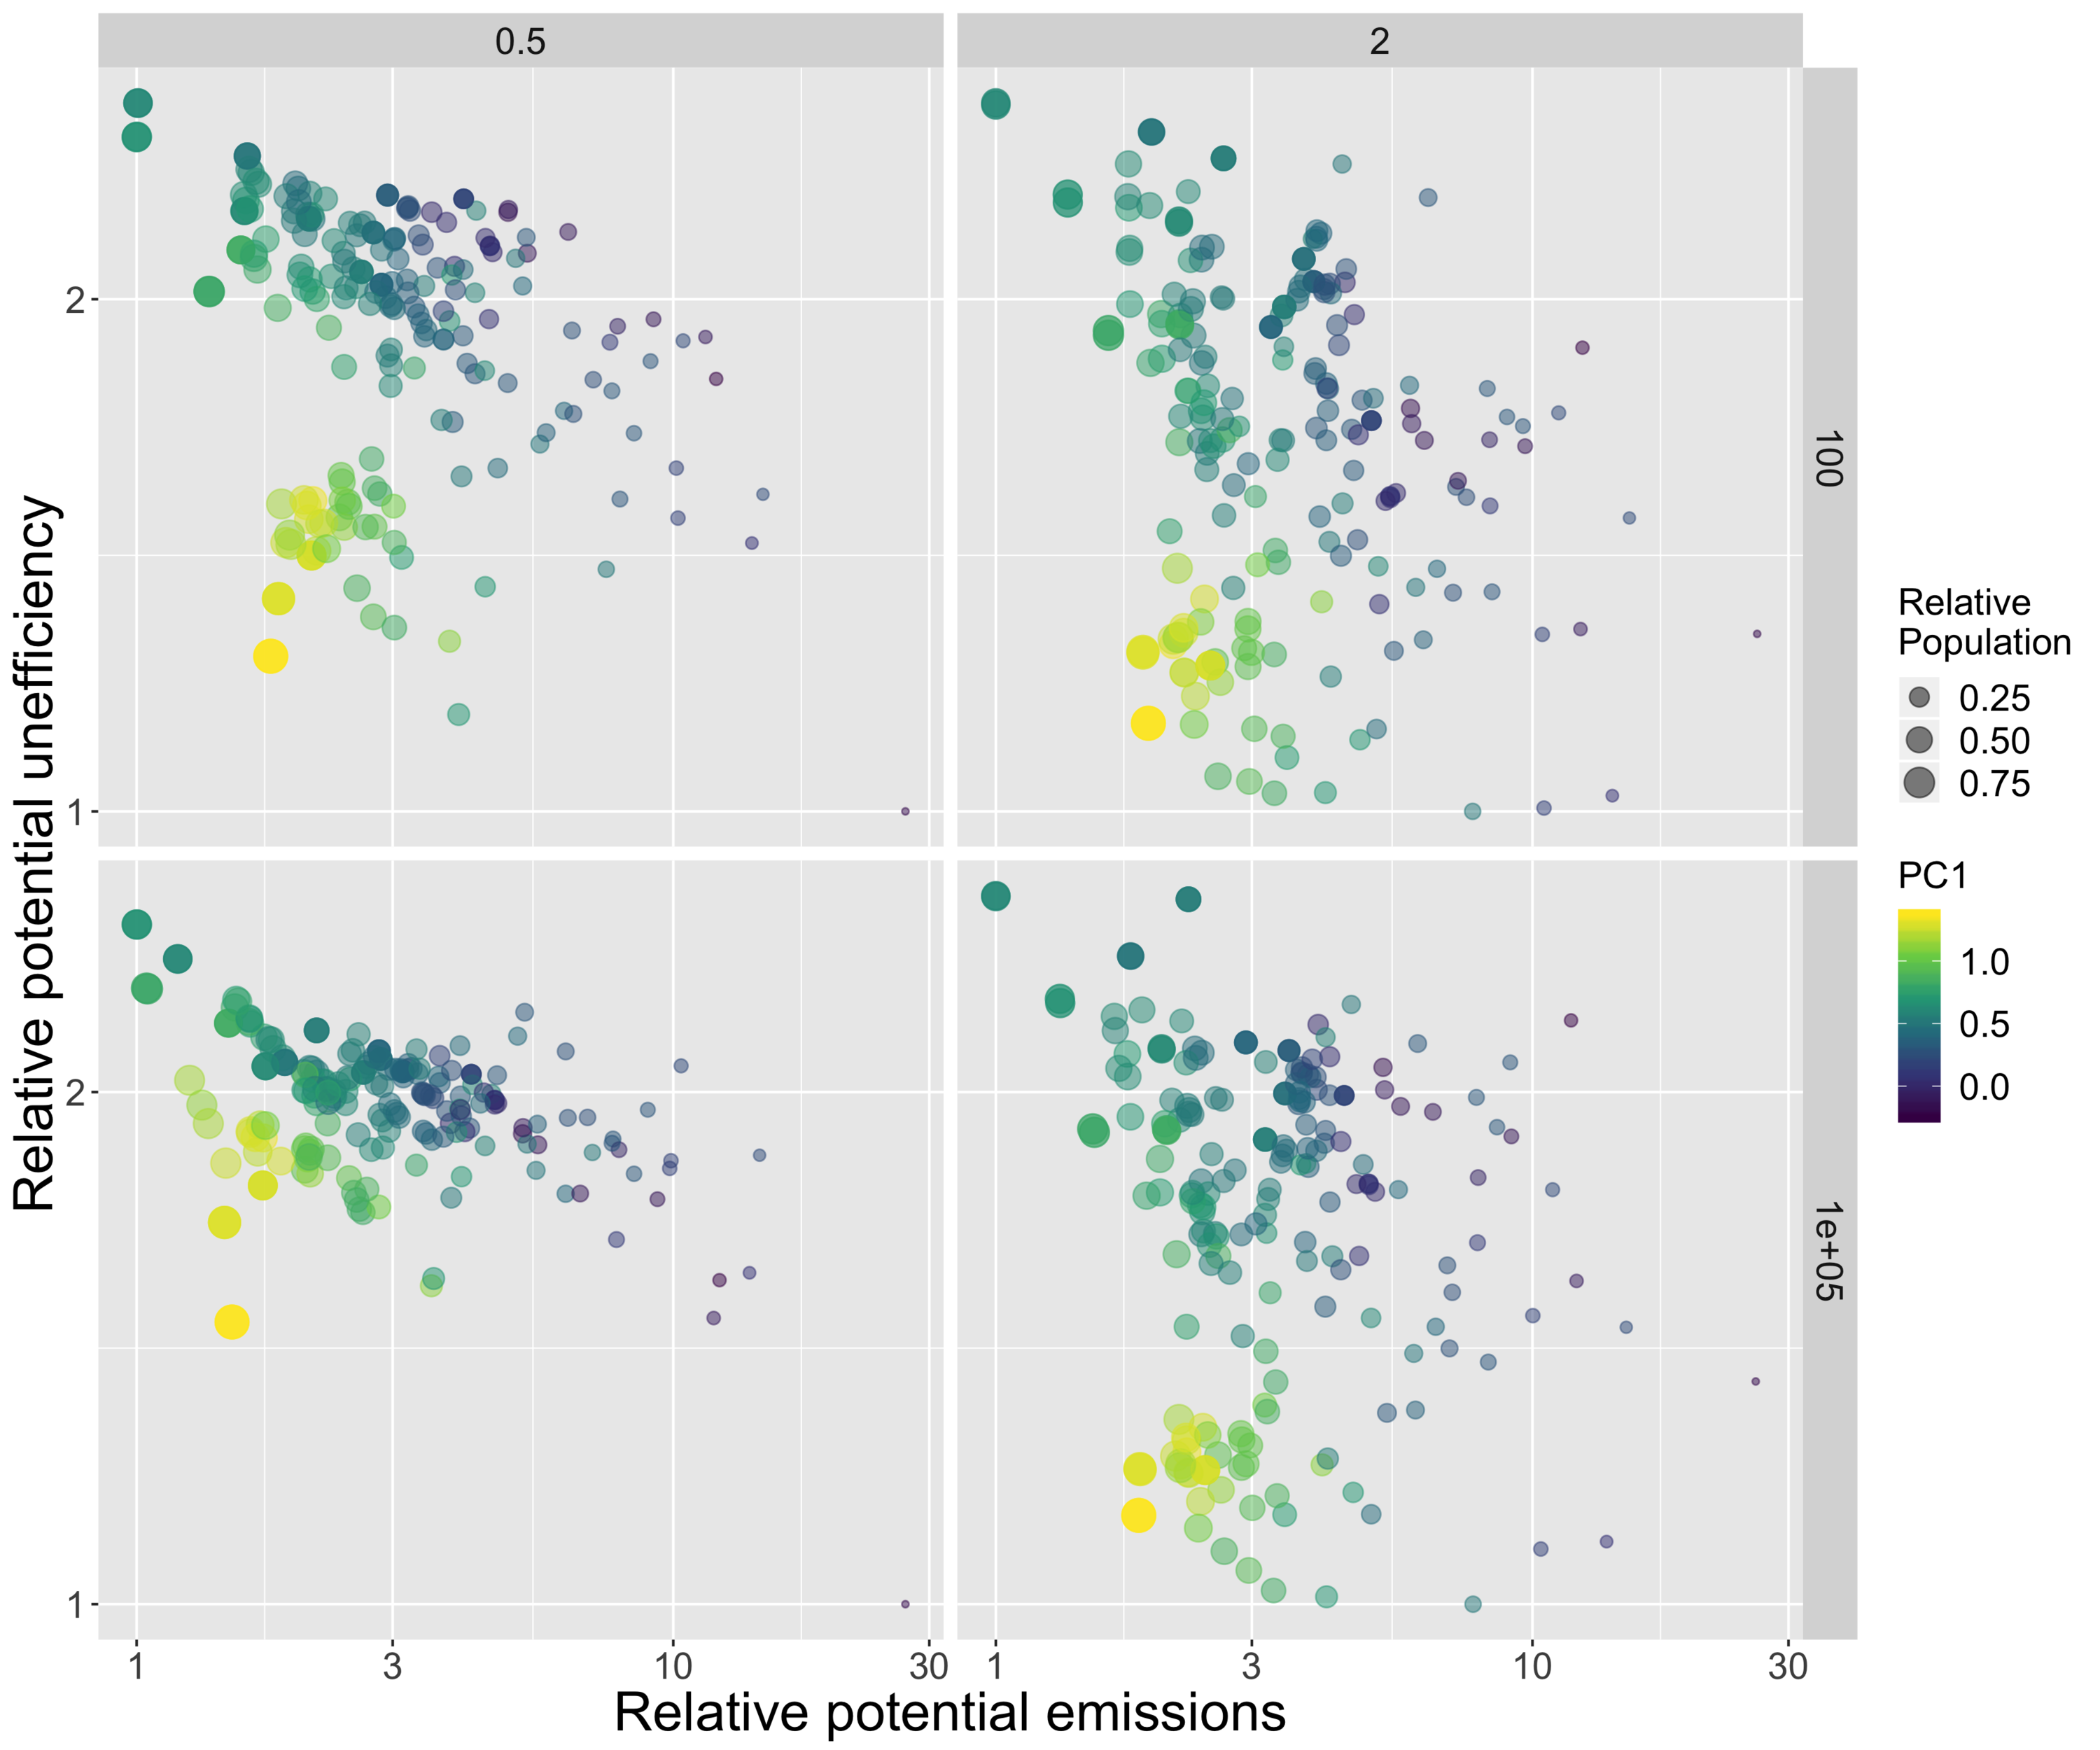
\includegraphics[width=\linewidth]{Fig7.png}}
  \centering  
  \caption{Relative potential emissions $\sum_c g_c$ against relative potential economic unefficiency $\sum_c e_c$ (both indicators should be minimized), for varying values of $\gamma_G$ (columns) and $d_G$ (rows). Color level gives the value of PC1, whereas point size gives the share of total population contained within considered areas.\label{fig:paretos-relative}}
\end{figure*}
%%%%%%%%%%%%%%%%%%%%


%%%%%%%%%%%%%
\subsection{Linking urban morphology and sustainability}


We now consider the sustainability indicators, aggregated for a configuration on all clusters. An important question is how these relate with measures of urban form \citep{le2012urban}. For a given parametrization of endogenous city regions, one can relate them to morphological indicators for population density spatial distribution. Such indicators were computed by~\cite{raimbault2018calibration}, and capture different dimensions of the spatial distribution of population, such as spatial autocorrelation (Moran index), homogeneity (entropy index), hierarchy (rank-size exponent), or level of aggregation (average distance between individuals). We average them here on clusters. This establishes a link between urban morphology and sustainibility. A principal component analysis on considered points yield 96\% of variance with two components, and 73\% explained by the first component alone. The first component relates to a level of monocentricity ($PC1 = -0.3\cdot I + 0.54 \cdot \bar{d} + 0.51\cdot \varepsilon + 0.59 \cdot h$ where $I$ is Moran index, $\bar{d}$ average distance, $\epsilon$ entropy, and $h$ level of hierarchy). In a nutshell, the principal dimension of urban form in differentiating our urban clusters is the level of monocentricity. We can relate it with indicators for emissions and economic efficiency.


We show in Fig.~\ref{fig:emissions-pc1} the value of $\sum_c \tilde{g}_c$ as a function of the first morphological principal component, for extreme values of $\gamma$ and $d_0$. There seems to exist an optimal intermediate value for PC1 regarding the minimization of normalized indicator for emissions only. This would correspond to an intermediate level of monocentricity, meaning that urban areas which are too polycentric and spread would emit more, but also areas that are too much monocentric. This behavior does not occur for long-range $d_0 = 100$km and low-hierarchy $\gamma=0.5$ interactions. The mostly monocentric but emitting configurations capture most of population (given by the level of color), whereas the intermediate configuration capture around half of the population, what means that these low-emissions potential urban regions can cover a significant part of European population.


However, when considering both emissions and economic indicators, urban form then acts as a compromise variable. We show in Fig.~\ref{fig:paretos-relative} the point clouds of $\sum_c g_c$ against $\sum_c e_c$, which produce clear Pareto fronts, which shape varies with $\gamma$ and $d_0$. As the color level gives the value of PC1, we can see the points on the different fronts with very different morphological properties. In some cases, highly monocentric areas (yellow points) can be a good compromise, whereas the intermediate optimal for emissions shown before may yield highly inefficient areas (dominated green points). For example, considering the fronts for $\gamma = 2$ which have both very similar shape, the points with the lowest emissions are on the top-left of the front and correspond to the optimal unveiled in Fig.~\ref{fig:emissions-pc1}. These have however a very low economic efficiency (high inefficiency) and small improvements can be done with the points below, before switching to a totally different urban form with a high value of PC1 (yellow points, highly monocentric). Increasing more the economic efficiency is then at the price of much more emissions, with more polycentric areas. This analysis therefore unveils morphological trade-offs, confirming that there is no optimal urban form, but different compromises regarding the conflicting sustainability indicators.



%%%%%%%%%%%%%%%%%
\section{Discussion}


\subsection{From multi-dimensional percolation to the sustainability of mega-city regions}

From the methodological point of view, we showed that network percolation can successfully be applied to multidimensional urban networks. This requires a consistent overlay within the same nodes of the different dimensions considered. The existence of percolation transitions which are different to the unidimensional case confirms that the approach captures complementary information, and that it could be applied to characterize urban systems in a more refined way. The non-existence of a significant maximum for the fractal dimension remains to be investigated, since it could be due a bias of our abstract network construction. Studies on other dimensions or on non-abstract networks remain to be done to understand how multi-dimensional percolation differs from the unidimensional one.


Regarding the second axis of our research question, we showed that multi-dimensional percolation is a useful tool to extract endogenous mega-urban regions while taking into account complementary aspects of population distribution and performance of transportation networks. Varying the parameters of the percolation algorithm provides a comparative view on possible clustering structures for the European urban system, and corresponding performance in terms of stylized sustainability indicators. Indeed, this work is exploratory in terms of possible definitions of urban subsystems. The fact that some systems obtained coincide with effective functional regions \citep{hall2006polycentric} shows that some thresholds of population and road network performance intensity capture actual functional linkages. This correspondance could not be predicted a priori nor explained through simple arguments as our approach reconstructs clusters from the bottom-up. Finally, the links between urban form and sustainability indicators made in the last section are also interesting for the management of urban systems, suggesting a certain performance of polycentric systems in particular regarding emissions.


%%%%%%%%%%%%%%%%%
\subsection{Developments}

Further work may consist in the use of calibration heuristics to find in a more robust way optimal parameter values. The OpenMOLE model exploration platform provides a transparent access to genetic algorithms for multi-objective optimization \citep{reuillon2013openmole}. The use of such calibration algorithms would allow to unveil the effective form of Pareto fronts, that we may have missed here through the grid sampling.


An other development would consist in extrapolating transportation flows with a spatially explicit gravity and transportation flow model as a kind of simplified four step model \citep{mcnally2000four}. It could then be adjusted on actual transportation flows emissions database which are also available in the Edgar database. The corresponding gravity parameters could then be used within the economic and emissions potentials, and the sustainability patterns produced compared with the hypothetical ones we produced here.

Finally, an important development would imply crossing our endogenous definitions of urban regions with socio-economic databases, and compute indicators implied in other dimensions of sustainability, for example related to socio-economic inequalities, spatial distribution of accessibilities, or activities with different scaling exponents. This includes the mitigation of spatial inequalities and segregation \citep{tammaru2015multi}, which are an important dimension of sustainability.



%%%%%%%%%%%%%%%%%
\subsection{Towards policy applications}


Our work suggests the possibility to design policies in terms of regional integration to increase the sustainability of mega-city regions. The way such results could actually be transferred to policy-making recommandations remains an open question, but Pareto-optimal configurations can be used for the planning of regional transportation networks for example, or to design policies for the distribution of subsidies. Indeed, privileging some infrastructure developments but also collaborations between urban centers can be seen as an aspect of a small scale planning, or territorial strategy. As we integrated potential flows that would result from such development, and consider their economic and emissions consequences, and did it in an endogenous way, we suggest that evidence-based strategies for territorial development at the European level could be inspired by this work. This would naturally imply a more thorough data integration, model calibration and operationalization.

  

%%%%%%%%%%%%%%%%%
\section{Conclusion}


In conclusion, our multilayer percolation approach captures in a way the multi-dimensionality of urban systems and a link between form and function in urban system. In particular, in our application on the bilayer case of an abstract network constructed from population density and road network indicators, it is shown to capture a different structure than in the unidimensional case. Its application to the issue of sustainable mega-city regions show how its properties of constructing urban clusters from the bottom-up can be used to study sustainability issues. This work also illustrates the importance of following data-driven paradigms even when developing, as what is understood of the behavior of the heuristic is through its application to real data and issues.



\section*{Acknowledgment}

This work is part of DynamiCity, a FUI project funded by BPI France, Auvergne-Rh{\^o}ne-Alpes region, Ile-de-France region and Lyon metropolis.



\begin{thebibliography}{}

\bibitem[\protect\citeauthoryear{Aleta and Moreno}{Aleta and
  Moreno}{2018}]{aleta2018multilayer}
Aleta A., Moreno Y. (2018).
\newblock Multilayer networks in a nutshell.
\newblock {\em Annual Review of Condensed Matter Physics\/}.


\bibitem[\protect\citeauthoryear{Arbabi, Mayfield, and McCann}{Arbabi
  \textit{et~al.}}{2019}]{arbabi2019development}
Arbabi H., Mayfield M., McCann P. (2019).
\newblock On the development logic of city-regions: inter-versus intra-city
  mobility in england and wales.
\newblock {\em Spatial Economic Analysis\/}, 1--20.


\bibitem[\protect\citeauthoryear{Arcaute, Molinero, Hatna, Murcio, Vargas-Ruiz,
  Masucci, and Batty}{Arcaute \textit{et~al.}}{2016}]{arcaute2016cities}
Arcaute E., Molinero C., Hatna E., Murcio R., Vargas-Ruiz C., Masucci A.~P.,
  Batty M. (2016).
\newblock Cities and regions in britain through hierarchical percolation.
\newblock {\em Royal Society open science\/}~{\em 3\/}(4), 150691.


\bibitem[\protect\citeauthoryear{Banos and Genre-Grandpierre}{Banos and
  Genre-Grandpierre}{2012}]{banos2012towards}
Banos A., Genre-Grandpierre C. (2012).
\newblock Towards new metrics for urban road networks: Some preliminary
  evidence from agent-based simulations.
\newblock In {\em Agent-based models of geographical systems}, pp.\  627--641.
  Springer.


\bibitem[\protect\citeauthoryear{Barth{\'e}lemy}{Barth{\'e}lemy}{2011}]{barthelemy2011spatial}
Barth{\'e}lemy M. (2011).
\newblock Spatial networks.
\newblock {\em Physics Reports\/}~{\em 499\/}(1-3), 1--101.


\bibitem[\protect\citeauthoryear{Batty and Longley}{Batty and
  Longley}{1994}]{batty1994fractal}
Batty M., Longley P.~A. (1994).
\newblock {\em Fractal cities: a geometry of form and function}.
\newblock Academic press.


\bibitem[\protect\citeauthoryear{Bettencourt, Lobo, Helbing, K{\"u}hnert, and
  West}{Bettencourt \textit{et~al.}}{2007}]{bettencourt2007growth}
Bettencourt L.~M., Lobo J., Helbing D., K{\"u}hnert C., West G.~B. (2007).
\newblock Growth, innovation, scaling, and the pace of life in cities.
\newblock {\em Proceedings of the national academy of sciences\/}~{\em
  104\/}(17), 7301--7306.


\bibitem[\protect\citeauthoryear{Boccaletti, Bianconi, Criado, Del~Genio,
  G{\'o}mez-Gardenes, Romance, Sendina-Nadal, Wang, and Zanin}{Boccaletti
  \textit{et~al.}}{2014}]{boccaletti2014structure}
Boccaletti S., Bianconi G., Criado R., Del~Genio C.~I., G{\'o}mez-Gardenes J.,
  Romance M., Sendina-Nadal I., Wang Z., Zanin M. (2014).
\newblock The structure and dynamics of multilayer networks.
\newblock {\em Physics Reports\/}~{\em 544\/}(1), 1--122.


\bibitem[\protect\citeauthoryear{Burger and Meijers}{Burger and
  Meijers}{2012}]{burger2012form}
Burger M., Meijers E. (2012).
\newblock Form follows function? linking morphological and functional
  polycentricity.
\newblock {\em Urban studies\/}~{\em 49\/}(5), 1127--1149.


\bibitem[\protect\citeauthoryear{Callaway, Newman, Strogatz, and
  Watts}{Callaway \textit{et~al.}}{2000}]{callaway2000network}
Callaway D.~S., Newman M.~E., Strogatz S.~H., Watts D.~J. (2000).
\newblock Network robustness and fragility: Percolation on random graphs.
\newblock {\em Physical review letters\/}~{\em 85\/}(25), 5468.


\bibitem[\protect\citeauthoryear{Cottineau, Finance, Hatna, Arcaute, and
  Batty}{Cottineau \textit{et~al.}}{2018}]{cottineau2018defining}
Cottineau C., Finance O., Hatna E., Arcaute E., Batty M. (2018).
\newblock Defining urban clusters to detect agglomeration economies.
\newblock {\em Environment and Planning B: Urban Analytics and City Science\/},
  2399808318755146.


\bibitem[\protect\citeauthoryear{Cottineau, Hatna, Arcaute, and
  Batty}{Cottineau \textit{et~al.}}{2017}]{cottineau2017diverse}
Cottineau C., Hatna E., Arcaute E., Batty M. (2017).
\newblock Diverse cities or the systematic paradox of urban scaling laws.
\newblock {\em Computers, environment and urban systems\/}~{\em 63}, 80--94.


\bibitem[\protect\citeauthoryear{Crucitti, Latora, and Porta}{Crucitti
  \textit{et~al.}}{2006}]{crucitti2006centrality}
Crucitti P., Latora V., Porta S. (2006).
\newblock Centrality measures in spatial networks of urban streets.
\newblock {\em Physical Review E\/}~{\em 73\/}(3), 036125.


\bibitem[\protect\citeauthoryear{Ducruet and Beauguitte}{Ducruet and
  Beauguitte}{2014}]{ducruet2014spatial}
Ducruet C., Beauguitte L. (2014).
\newblock Spatial science and network science: Review and outcomes of a complex
  relationship.
\newblock {\em Networks and Spatial Economics\/}~{\em 14\/}(3-4), 297--316.


\bibitem[\protect\citeauthoryear{Feng, Wu, Wu, Su, Weng, and Bian}{Feng
  \textit{et~al.}}{2018}]{feng2018spatiotemporal}
Feng Y., Wu S., Wu P., Su S., Weng M., Bian M. (2018).
\newblock Spatiotemporal characterization of megaregional poly-centrality:
  Evidence for new urban hypotheses and implications for polycentric policies.
\newblock {\em Land use policy\/}~{\em 77}, 712--731.


\bibitem[\protect\citeauthoryear{Florida, Gulden, and Mellander}{Florida
  \textit{et~al.}}{2008}]{florida2008rise}
Florida R., Gulden T., Mellander C. (2008).
\newblock The rise of the mega-region.
\newblock {\em Cambridge Journal of Regions, Economy and Society\/}~{\em
  1\/}(3), 459--476.


\bibitem[\protect\citeauthoryear{Hackett, Cellai, G{\'o}mez, Arenas, and
  Gleeson}{Hackett \textit{et~al.}}{2016}]{hackett2016bond}
Hackett A., Cellai D., G{\'o}mez S., Arenas A., Gleeson J.~P. (2016).
\newblock Bond percolation on multiplex networks.
\newblock {\em Physical Review X\/}~{\em 6\/}(2), 021002.


\bibitem[\protect\citeauthoryear{Hall and Pain}{Hall and
  Pain}{2006}]{hall2006polycentric}
Hall P.~G., Pain K. (2006).
\newblock {\em The polycentric metropolis: learning from mega-city regions in
  Europe}.
\newblock Routledge.


\bibitem[\protect\citeauthoryear{Hillier, Leaman, Stansall, and
  Bedford}{Hillier \textit{et~al.}}{1976}]{hillier1976space}
Hillier B., Leaman A., Stansall P., Bedford M. (1976).
\newblock Space syntax.
\newblock {\em Environment and Planning B: Planning and design\/}~{\em 3\/}(2),
  147--185.


\bibitem[\protect\citeauthoryear{Huynh, Makarov, Legara, Monterola, and
  Chew}{Huynh \textit{et~al.}}{2018}]{huynh2018characterisation}
Huynh H.~N., Makarov E., Legara E.~F., Monterola C., Chew L.~Y. (2018).
\newblock Characterisation and comparison of spatial patterns in urban systems:
  A case study of us cities.
\newblock {\em Journal of computational science\/}~{\em 24}, 34--43.


\bibitem[\protect\citeauthoryear{Janssens-Maenhout, Crippa, Guizzardi, Muntean,
  Schaaf, Dentener, Bergamaschi, Pagliari, Olivier, Peters,
  \textit{et~al.}}{Janssens-Maenhout \textit{et~al.}}{2017}]{janssens2017edgar}
Janssens-Maenhout G., Crippa M., Guizzardi D., Muntean M., Schaaf E., Dentener
  F., Bergamaschi P., Pagliari V., Olivier J., Peters J., \textit{et~al.}
  (2017).
\newblock Edgar v4. 3.2 global atlas of the three major greenhouse gas
  emissions for the period 1970--2012.
\newblock {\em Earth Syst. Sci. Data Discuss\/}.


\bibitem[\protect\citeauthoryear{Komiyama and Takeuchi}{Komiyama and
  Takeuchi}{2006}]{komiyama2006sustainability}
Komiyama H., Takeuchi K. (2006).
\newblock {\em Sustainability science: building a new discipline}.


\bibitem[\protect\citeauthoryear{Lagesse, Bordin, and Douady}{Lagesse
  \textit{et~al.}}{2015}]{lagesse2015spatial}
Lagesse C., Bordin P., Douady S. (2015).
\newblock A spatial multi-scale object to analyze road networks.
\newblock {\em Network Science\/}~{\em 3\/}(1), 156--181.


\bibitem[\protect\citeauthoryear{Lang and Dhavale}{Lang and
  Dhavale}{2005}]{lang2005beyond}
Lang R.~E., Dhavale D. (2005).
\newblock Beyond megalopolis: Exploring america’s new “megapolitan”
  geography.


\bibitem[\protect\citeauthoryear{Laquian}{Laquian}{2011}]{laquian2011planning}
Laquian A. (2011).
\newblock The planning and governance of asia’s mega-urban regions.
\newblock {\em Population Distribution, Urbanization, Internal Migration and
  Development: An International Perspective, United Nations Department of
  Economic and Social Affairs, Population Division, New York: United
  Nations\/}, 302--322.


\bibitem[\protect\citeauthoryear{Lashof and Ahuja}{Lashof and
  Ahuja}{1990}]{lashof1990relative}
Lashof D.~A., Ahuja D.~R. (1990).
\newblock Relative contributions of greenhouse gas emissions to global warming.
\newblock {\em Nature\/}~{\em 344\/}(6266), 529.


\bibitem[\protect\citeauthoryear{Le~N{\'e}chet}{Le~N{\'e}chet}{2012}]{le2012urban}
Le~N{\'e}chet F. (2012).
\newblock Urban spatial structure, daily mobility and energy consumption: a
  study of 34 european cities.
\newblock {\em Cybergeo: European Journal of Geography\/}.


\bibitem[\protect\citeauthoryear{Le~N{\'e}chet}{Le~N{\'e}chet}{2017}]{lenechet2017peupler}
Le~N{\'e}chet F. (2017).
\newblock De l'{\'e}talement urbain aux r{\'e}gions m{\'e}tropolitaines
  polycentriques : formes de fonctionnement et formes de gouvernance.
\newblock In {\em {Peupler la terre - De la pr{\'e}histoire {\`a} l'{\`e}re des
  m{\'e}tropoles}}. Presses Universitaires Francois Rabelais.


\bibitem[\protect\citeauthoryear{Li, Fu, Wang, Lu, Berezin, Stanley, and
  Havlin}{Li \textit{et~al.}}{2015}]{Li669}
Li D., Fu B., Wang Y., Lu G., Berezin Y., Stanley H.~E., Havlin S. (2015).
\newblock Percolation transition in dynamical traffic network with evolving
  critical bottlenecks.
\newblock {\em Proceedings of the National Academy of Sciences\/}~{\em
  112\/}(3), 669--672.
\newblock URL: \url{https://www.pnas.org/content/112/3/669}, \href
  {http://arxiv.org/abs/https://www.pnas.org/content/112/3/669.full.pdf}
  {arXiv:https://www.pnas.org/content/112/3/669.full.pdf}, \href
  {http://dx.doi.org/10.1073/pnas.1419185112} {doi:10.1073/pnas.1419185112}.


\bibitem[\protect\citeauthoryear{Louf and Barthelemy}{Louf and
  Barthelemy}{2013}]{louf2013modeling}
Louf R., Barthelemy M. (2013).
\newblock Modeling the polycentric transition of cities.
\newblock {\em Physical review letters\/}~{\em 111\/}(19), 198702.


\bibitem[\protect\citeauthoryear{Makse, Andrade, Batty, Havlin, Stanley,
  \textit{et~al.}}{Makse \textit{et~al.}}{1998}]{makse1998modeling}
Makse H.~A., Andrade J.~S., Batty M., Havlin S., Stanley H.~E., \textit{et~al.}
  (1998).
\newblock Modeling urban growth patterns with correlated percolation.
\newblock {\em Physical Review E\/}~{\em 58\/}(6), 7054.


\bibitem[\protect\citeauthoryear{Marull, Galletto, Domene, and
  Trull{\'e}n}{Marull \textit{et~al.}}{2013}]{marull2013emerging}
Marull J., Galletto V., Domene E., Trull{\'e}n J. (2013).
\newblock Emerging megaregions: a new spatial scale to explore urban
  sustainability.
\newblock {\em Land Use Policy\/}~{\em 34}, 353--366.


\bibitem[\protect\citeauthoryear{McNally}{McNally}{2000}]{mcnally2000four}
McNally M.~G. (2000).
\newblock The four step model.


\bibitem[\protect\citeauthoryear{Newman and Watts}{Newman and
  Watts}{1999}]{newman1999scaling}
Newman M.~E., Watts D.~J. (1999).
\newblock Scaling and percolation in the small-world network model.
\newblock {\em Physical review E\/}~{\em 60\/}(6), 7332.


\bibitem[\protect\citeauthoryear{Offner, Beaucire, Delaplace, Fr{\'e}mont,
  Ninot, Bretagnolle, and Pumain}{Offner
  \textit{et~al.}}{2014}]{espacegeo2014effets}
Offner J.-M., Beaucire F., Delaplace M., Fr{\'e}mont A., Ninot O., Bretagnolle
  A., Pumain D. (2014).
\newblock Les effets structurants des infrastructures de transport.
\newblock {\em Espace Geographique\/}~(42), p--51.


\bibitem[\protect\citeauthoryear{Penrose}{Penrose}{1999}]{penrose1999k}
Penrose M.~D. (1999).
\newblock On k-connectivity for a geometric random graph.
\newblock {\em Random Structures \& Algorithms\/}~{\em 15\/}(2), 145--164.


\bibitem[\protect\citeauthoryear{Perez, Banos, and Pettit}{Perez
  \textit{et~al.}}{2016}]{perez2016agent}
Perez P., Banos A., Pettit C. (2016).
\newblock Agent-based modelling for urban planning current limitations and
  future trends.
\newblock In {\em International Workshop on Agent Based Modelling of Urban
  Systems}, pp.\  60--69. Springer.


\bibitem[\protect\citeauthoryear{Piovani, Molinero, and Wilson}{Piovani
  \textit{et~al.}}{2017}]{piovani2017urban}
Piovani D., Molinero C., Wilson A. (2017).
\newblock Urban retail location: insights from percolation theory and spatial
  interaction modeling.
\newblock {\em PloS one\/}~{\em 12\/}(10), e0185787.


\bibitem[\protect\citeauthoryear{Raimbault}{Raimbault}{2018a}]{raimbault2018calibration}
Raimbault J. (2018a).
\newblock Calibration of a density-based model of urban morphogenesis.
\newblock {\em PloS one\/}~{\em 13\/}(9), e0203516.


\bibitem[\protect\citeauthoryear{Raimbault}{Raimbault}{2018b}]{raimbault2018caracterisation}
Raimbault J. (2018b).
\newblock {\em Caract{\'e}risation et mod{\'e}lisation de la co-{\'e}volution
  des r{\'e}seaux de transport et des territoires}.
\newblock Ph.\ D. thesis, Universit{\'e} Paris 7 Denis Diderot.


\bibitem[\protect\citeauthoryear{Raimbault}{Raimbault}{2018c}]{raimbault2018indirect}
Raimbault J. (2018c).
\newblock Indirect evidence of network effects in a system of cities.
\newblock {\em Environment and Planning B: Urban Analytics and City Science\/},
  2399808318774335.


\bibitem[\protect\citeauthoryear{Raimbault}{Raimbault}{2019}]{raimbault2018urban}
Raimbault J. (2019).
\newblock An urban morphogenesis model capturing interactions between networks
  and territories.
\newblock In {\em The Mathematics of Urban Morphology}, pp.\  383--409.
  Springer.


\bibitem[\protect\citeauthoryear{Reuillon, Leclaire, and
  Rey-Coyrehourcq}{Reuillon \textit{et~al.}}{2013}]{reuillon2013openmole}
Reuillon R., Leclaire M., Rey-Coyrehourcq S. (2013).
\newblock Openmole, a workflow engine specifically tailored for the distributed
  exploration of simulation models.
\newblock {\em Future Generation Computer Systems\/}~{\em 29\/}(8), 1981--1990.


\bibitem[\protect\citeauthoryear{Sanders}{Sanders}{2017}]{sanders2017peupler}
Sanders L. (2017).
\newblock {\em Peupler la terre - De la pr{\'e}histoire {\`a} l'{\`e}re des
  m{\'e}tropoles.}
\newblock Presses Universitaires Francois Rabelais.


\bibitem[\protect\citeauthoryear{Son, Bizhani, Christensen, Grassberger, and
  Paczuski}{Son \textit{et~al.}}{2012}]{son2012percolation}
Son S.-W., Bizhani G., Christensen C., Grassberger P., Paczuski M. (2012).
\newblock Percolation theory on interdependent networks based on epidemic
  spreading.
\newblock {\em EPL (Europhysics Letters)\/}~{\em 97\/}(1), 16006.


\bibitem[\protect\citeauthoryear{Sorensen and Okata}{Sorensen and
  Okata}{2010}]{sorensen2010megacities}
Sorensen A., Okata J. (2010).
\newblock {\em Megacities: Urban form, governance, and sustainability},
  Volume~10.
\newblock Springer Science \& Business Media.


\bibitem[\protect\citeauthoryear{Stauffer and Aharony}{Stauffer and
  Aharony}{2014}]{stauffer2014introduction}
Stauffer D., Aharony A. (2014).
\newblock {\em Introduction to percolation theory}.
\newblock Taylor \& Francis.


\bibitem[\protect\citeauthoryear{Su, Liu, Xu, Li, Pi, and Weng}{Su
  \textit{et~al.}}{2017}]{su2017china}
Su S., Liu Z., Xu Y., Li J., Pi J., Weng M. (2017).
\newblock China’s megaregion policy: Performance evaluation framework,
  empirical findings and implications for spatial polycentric governance.
\newblock {\em Land Use Policy\/}~{\em 63}, 1--19.


\bibitem[\protect\citeauthoryear{Tammaru, Marci{\'n}czak, Van~Ham, and
  Musterd}{Tammaru \textit{et~al.}}{2015}]{tammaru2015multi}
Tammaru T., Marci{\'n}czak S., Van~Ham M., Musterd S. (2015).
\newblock A multi-factor approach to understanding socio-economic segregation
  in european capital cities.
\newblock In {\em Socio-economic segregation in European capital cities}, pp.\
  25--53. Routledge.


\bibitem[\protect\citeauthoryear{Tobler}{Tobler}{2004}]{tobler2004first}
Tobler W. (2004).
\newblock On the first law of geography: A reply.
\newblock {\em Annals of the Association of American Geographers\/}~{\em
  94\/}(2), 304--310.


\bibitem[\protect\citeauthoryear{Vigui{\'e} and Hallegatte}{Vigui{\'e} and
  Hallegatte}{2012}]{viguie2012trade}
Vigui{\'e} V., Hallegatte S. (2012).
\newblock Trade-offs and synergies in urban climate policies.
\newblock {\em Nature Climate Change\/}~{\em 2\/}(5), 334.


\bibitem[\protect\citeauthoryear{Zeng, Li, Guo, Gao, Gao, Stanley, and
  Havlin}{Zeng \textit{et~al.}}{2019}]{Zeng23}
Zeng G., Li D., Guo S., Gao L., Gao Z., Stanley H.~E., Havlin S. (2019).
\newblock Switch between critical percolation modes in city traffic dynamics.
\newblock {\em Proceedings of the National Academy of Sciences\/}~{\em
  116\/}(1), 23--28.


\end{thebibliography}




\end{document}
